\documentclass[times, utf8, diplomski]{fer}
\usepackage{booktabs}
\usepackage{listings}
\graphicspath{{./img/}}
\lstset{language=Python, tabsize=4, numbers=left, basicstyle=\small}

\begin{document}

% TODO: Navedite broj rada.
\thesisnumber{2451}

% TODO: Navedite naslov rada.
\title{Klasifikacija pokreta ljudskog tijela temeljena na podacima s inercijskih senzora}

% TODO: Navedite vaše ime i prezime.
\author{Ivan Trubić}

\maketitle

% Ispis stranice s napomenom o umetanju izvornika rada. Uklonite naredbu \izvornik ako želite izbaciti tu stranicu.
%\izvornik

% Dodavanje zahvale ili prazne stranice. Ako ne želite dodati zahvalu, naredbu ostavite radi prazne stranice.
\zahvala{}

\tableofcontents

\chapter{Uvod}
Karakteristike pokreta ljudskoga tijela vrlo su individualne te ovise o mnogo čimbenika kao što su genetika, odgoj te
fizička sprema. Ti pokreti su toliko jedinstveni da se mogu koristiti za identifikaciju osoba dok su, s druge strane,
toliko slični da čak i manje devijacije u tim pokretima također mogu ukazivati na neke zdravstvene probleme.
Ljudski pokreti mogu se klasificirati na razne načine koristeći računalni vid ili razne senzore postavljene na
ljudskome tijelu. Svaka od metoda ima svoju granu primjene kao: identifikacija osoba temeljenog na hodu koristeći
računalni vid na nadzornim kamerama \citep{surveillance}, praćenje pokreta igrača u interakciji s igrama u virtualnoj stvarnosti \citep{VR},
korištenje inercijskih (IMU) senzora za precizno snimanje hoda u svrhu otkrivanja bolesti i rehabilitacije te mnoge druge.

Klasifikacija pokreta vrlo je složen problem te kao takav nema dobro rješenje koristeći klasične algoritme. Razvojem moći računala
te metoda strojnoga učenja ovaj problem postaje rješiv. Za snimanje pokreta može se koristiti kamera ili senzori.
Koristeći kameru, na snimci se koriste metode računalnog vida te se traže karakteristike ljudskog tijela kako bi se na snimci
prepoznala osoba te koristeći te karakteristične točke analizira se hod. Također, kamera može snimati osobu s posebno postavljenim
vizualnim oznakama po dijelovima tijela te koristeći te vizualne oznake analizirati pokrete. Nedostatak kamera je taj što snimaju iz
jedne perspektive te zbog toga može doći do okluzije oznaka. Inercijski (IMU) senzori eliminiraju kamere te ne pate od problema okluzije.
Inercijski senzori su relativno jeftini i mali uređaji koji se postave na ključne dijelove ljudskoga tijela te pružaju vrlo dobar uvid
u ljudske pokrete. Primjerice mogu se staviti na ruke te upravljati igrama i uređajima ali se mogu koristiti i u medicinske svrhe za
analizu hoda i dijagnosticiranje zdravstvenih problema kao i za provođenje terapijskih vježbi bez nadzora stručnjaka.
Ovaj rad će se više fokusirati na medicinski aspekt klasifikacije pokreta, preciznije analizu hoda (\textit{eng.} gait) i terapiju koljena.


\chapter{Metode prikupljanja podataka}
Podaci o ljudskim pokretima mogu se prikupljati koristeći različite metode i tehnologije.
Svaka od tih tehnologija ima svoju granu primjene te možda neće biti adekvatna za primjenu u nekoj drugoj grani.

Prva razmatrana metoda prikupljanja informacija o pokretima je korištenje platformi sila. Platforme sila su elementi po kojima osoba
hoda te u sebi ima elastično mjerilo deformacija, odnosno tenzometrijski pretvornik prikazan na slici \ref{defgag}. 

\begin{figure}[h!]
    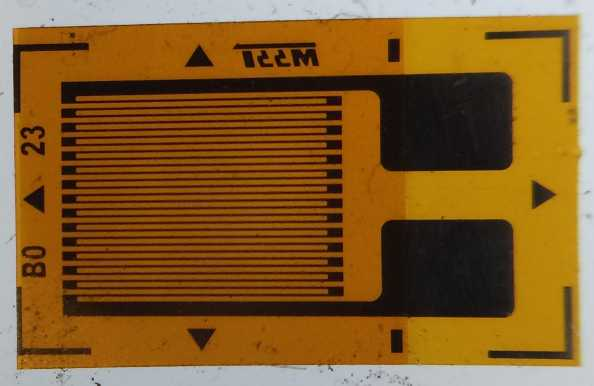
\includegraphics[width=\textwidth]{strain_gauge.jpg}
    \caption{Izgled mjerila deformacija (preuzeto sa \textit{wikipedia.com})}
    \label{defgag}
\end{figure}

Ovakvo mjerilo mjeri uzdužnu deformaciju tako da se elastični vodič prilikom deformacije produlji, odnosno skrati
čime se zbog produljenja i sužavanja, odnosno skraćivanja i širenja vodiča mijenja ukupan otpor i time se deformacija može izmjeriti.
Ovisno o arhitekturi mjerila on mjeri deformaciju u nekome smjeru te kombinacijom više mjerila može se izmjeriti deformacija
u sve tri osi. Na taj način može se dobiti GRFV (eng. \textit{Ground Reaction Force Vector}) koji predstavlja, prema trećem Newtonovom zakonu,
silu reakcije i suprotna je utjecaju osobe koja djeluje na ploču. Osim ovakvih mjerila deformacija mogu se koristiti piezoelektrici
koji svojom deformacijom stvaraju naboj koji se uz pomoć nabojskog pojačala pretvara u napon. Piezoelektrične platforme sila puno su preciznije ali su
i znatno skuplje te ovise o budžetu i o primjeni koja se tehnologija koristi. Ovakav pristup daje uvid isključivo u sile koje
djeluju na stopala i distribuciju težišta što je vrlo povoljno za analizu hoda ali ne i za druge primjene. Platforme sila vrlo su popularne
pri mjerenju performansi sportaša te mnoge profesionalne sportske ustanove i klubovi ulažu u vlastite ploče kako bi mogli nadzirati
svoje igrače. Ovakav pristup je korišten za prikupljanje jedne od najvećih baza podataka anotiranih za kliničku analizu \citep{pressurePlate}
opisanu u kasnijem poglavlju. Koristeći isto načelo, kako bi se lakše mogle pratiti sile koje djeluju na stopala prilikom
raznih aktivnosti, moguće je napraviti uloške za cipele koji su također mjerila sila. Na ovakav način moguće je pratiti korake
ispitanika bez postavljanja više velikih platformi sila te ograničavanja ispitanika na samo tu manju površinu što je za potrebe
praćenja performansi sportaša u pojedinim sportovima idealno.

Jedna od metoda koja služi baš praćenju pozicija donjih ekstremiteta je korištenje egzoskeleta. Egzoskelet je naprava koja se
postavi na vanjsku stranu ljudskoga tijela kako bi se njegovi dijelovi kretali skupa sa dijelovima tijela. Kako je svako tijelo
različitih dimenzija egzoskelet se mora moći namjestiti prema fizionomiji osobe na koju se postavlja kako bi zglobovi bili u
ravnini s osovinama egzoskeleta. Za snimanje kretanja, na osovine egzoskeleta se postavljaju promjenjivi otpornici koji te osovine
pretvaraju u goniometar - uređaj koji mjeri kuteve. Svaki pokret zgloba može se zapisati kao promjena otpora u vremenu. Za to je
potrebno imati osovine na području kukova, koljena i skočnih zglobova. Ovakav pristup puno vjernije snima pokrete tijela od platformi sila
jer se ne gleda samo sila reakcije podloge već se precizno mjere kutevi njegovih ekstremiteta u vremenu. 

Problem korištenja egzoskeleta je taj što sam egzoskelet može značajno promijeniti način kretanja. Razlog tome je masa egzoskeleta
koja ovisi o materijalima i izvedbi te način pričvršćivanja za ljudsko tijelo. Također promjenjivi otpornici snimaju kuteve 
ekstremiteta u samo jednoj ravnini te ne snimaju, niti konstrukcija dopušta, moguću rotaciju ekstremiteta u drugim smjerovima.
Egzoskeleti mogu poslužiti za snimanje pokreta no njihova prava primjena nije u domeni prikupljanja podataka. Njihova primjena 
leži u robotskim egzoskeletima kakav je, primjerice, na slici \ref{exoskeleton}.

\begin{figure}
    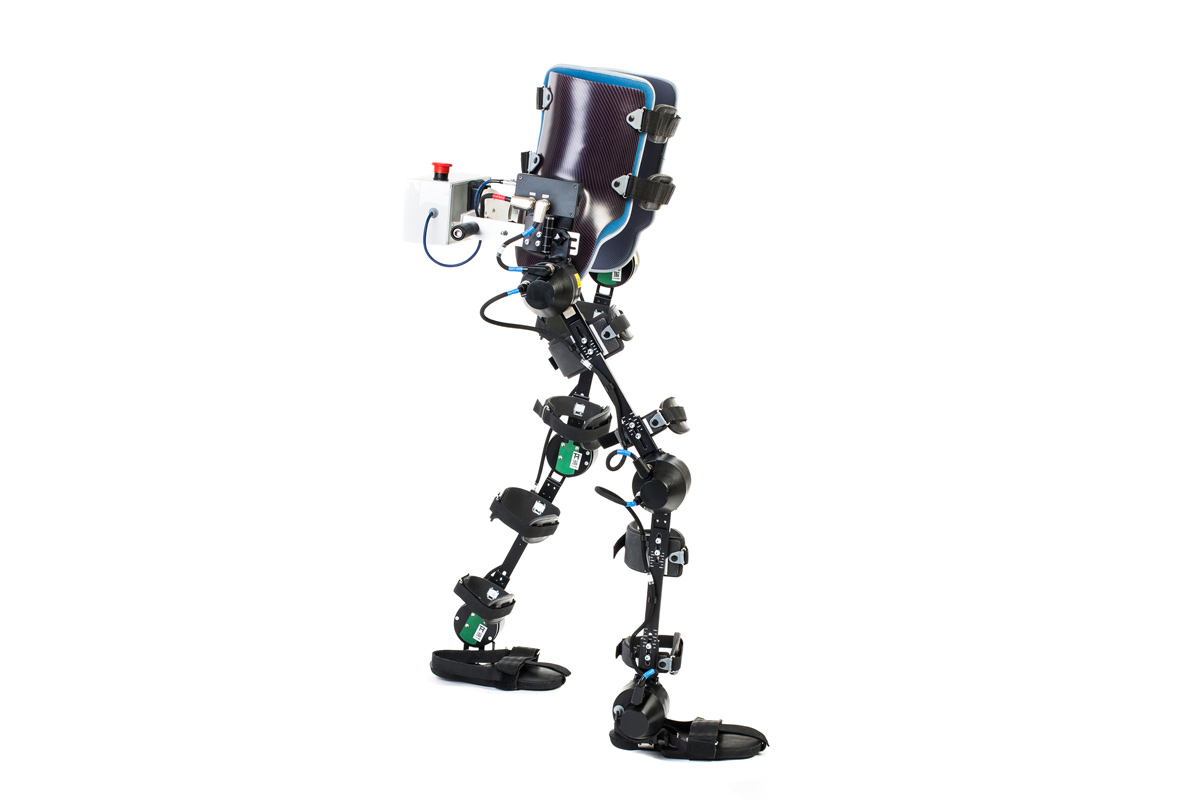
\includegraphics[width=\textwidth]{exoskeleton.jpg}
    \caption{Primjerak robotskog egzoskeleta Exo-H3 (preuzeto sa \textit{technaid.com})}
    \label{exoskeleton}
\end{figure}

Robotski egzoskeleti su naprave koje nemaju isključivo senzore i snimaju pokrete već uz senzore imaju i aktuatore kao elektromotore.
Aktuatori glume ljudske pokrete i pomažu osobama s poteškoćama. Jedna od glavnih primjena robotskih egzoskeleta je u fizikalnim
terapijama u kojima pacijenti zbog nekakve ozljede trebaju učiti ponovno hodati te pomažu nepokretnim osobama i osobama koje su
doživjele moždani udar da postanu i ostanu mobilni. Potencijal ovakvih robotskih egzoskeleta je uvidjela i vojna industrija te
je razvoj krenuo i u tom smjeru. U slučaju da osoba nije nepokretna moguće je iskoristiti senzore kako bi se pokreti snimali te
bi aktuatori istovremeno te pokrete izvodili \citep{exo}. Time se znatno rasterećuje ljudsko tijelo ali ovisno i o snazi aktuatora moguće je i
povećati ljudsku snagu. Na taj bi način jedna osoba mogla podizati predmete znatno teže nego što bi ona to sama ikad mogla
napraviti i to bez ikakvog naprezanja jer bi cijela težina predmeta bila raspoređena na strukturi egzoskeleta a ne na ljudskom 
tijelu što značajno rasterećuje tijelo te se osoba vremenom ne umara. Ovakva tehnologija se također razmatra za veliko unapređenje
radnih uvjeta u građevinskoj i logističkoj industriji jer bi se znatno umanjile nesreće uzrokovane padom predmeta zbog ljudskog
umora i očuvala ljudska tijela jer ne bi više dolazilo do ozljeda, primjerice dobivanja bruha zbog prevelikog tereta na tijelu.

Kako sam egzoskelet znatno utječe na slobodno kretanje udova sljedeća razmatrana metoda prikupljanja podataka taj problem pokušava riješiti
bez naprava koje bi smetale snimanju slobodnog pokreta. Digitalne kamere snimaju kretanje osobe te kako nisu pričvršćene na osobu
na nikakav način ne utječu na njeno kretanje stoga je osoba u mogućnosti kretati se na najprirodniji mogući način. Ovisno o količini
sličica u sekundi kojom kamera snima osobu može se dobiti brzo uzorkovanje, primjerice korištenjem vrlo brzih kamera s i do
12600 sličica u sekundi ili korištenjem standardnih potrošačkih kamera do 100 sličica u sekundi. Idući od sličice do sličice osoba ručno
može označiti karakteristične točke na ljudskome tijelu te na taj način doći do podataka no takav postupak bi bio vrlo iscrpljujuć i
nepraktičan. Za automatizaciju tog postupka može se iskoristiti nekoliko različitih metoda. Prva razmatrana će biti korištenje
računalnog vida. Računalni vid je grana računalne znanosti koja se bavi načinom na koji računalo obrađuje digitalne slike i video zapise 
te razumijeva njihov sadržaj. Za rješavanje ovakve problematike se izdvajaju zavidna sredstva te je istraživanje došlo vrlo daleko.
Kina je jedna od zemalja koja ulaže puno sredstava u tehnologiju računalnog vida jer joj je u interesu koristiti tehnologiju za 
masovni nadzor građana. Snimke s kamere se analiziraju te je algoritam u mogućnosti prepoznati točnu osobu koja se na 
snimci nalazi u stvarnome vremenu. Na sličan način je moguće na snimci prepoznati ljudsko tijelo te označiti interesne točke kao zglobove ekstremiteta
te na taj način automatizirano prikupiti podatke o karakteristikama pokreta. Problem ovoga pristupa je ovisnost o osvjetljenju i o
dovoljno velikom kontrastu između osobe i pozadine kako bi algoritam pronašao željene točke. U slučaju da je kontrast suviše mali, 
algoritam neće biti u mogućnosti prepoznati osobu ni interesne točke na snimci. Kada su laboratorijski uvjeti mogući, koristi se
kombinacija pozadine i odjeće koja je vrlo kontrastna te koristeći jednostavnu obradu slike moguće je izdvojiti samu siluetu osobe
što znatno poboljšava rezultate algoritma i prepoznavanje pokreta.

Za povećanje preciznosti praćenja pokreta moguće je koristiti sljedeću razmatranu metodu, a to je korištenje reflektirajućih markera
prilikom snimanja. Reflektirajući markeri su napravljeni po mogućnosti od retroreflektirajućih materijala (često poznatih pod nazivom
\textit{mačje oko}) koji iz bilo kojeg kuta
mogu reflektirati izvor svjetlosti u istom smjeru iz kojega ta svjetlost dolazi za razliku od zrcala koja reflektiraju svjetlost u ovisnosti o
upadnome kutu. Za potrebe snimanja takvih markera izvor svjetlosti se nalazi pored objektiva kamere te markeri postavljeni na
ljudsko tijelo daju vrlo dobru oznaku traženih točaka.
Prilikom obrade snimke te markere je vrlo lako izdvojiti jer su znatno svjetliji od svoje okoline te se na taj način može dobiti
vrlo precizna snimka pozicija tih točaka u prostoru. Kako bi ti markeri predstavljali dio tijela što preciznije potrebno ih je
postaviti na vrlo usku odjeću kako bi se kretali točno s tijelom bez dodatnih smetnji koje bi kretanje tkanine proizvelo. Također,
kako se što većim kontrastom lakše detektiraju, ti markeri trebaju biti postavljeni na tamnu odjeću, ovisno o primjeni crnu ili
sivu. Za još bolje rezultate mogu
se i iskoristiti i \textbf{aktivni} markeri koji su, u suštini, LED diode te emitiraju svjetlost što znači da ne ovisi o dodatnome
osvjetljenju za razliku od \textit{pasivnih} (reflektirajućih) markera koji samo reflektiraju već postojeće svjetlo. Ovakav pristup dopušta
postavljanje i praćenje proizvoljnog broja točaka na ljudskome tijelu. Jedini uvjet je da te točke budu dovoljno razmaknute jedne
od drugih kako bi kamera sa svoje udaljenosti mogla razlikovati svaku točku posebno. Kako je kamera uređaj koji snima dvodimenzionalnu
sliku iz perspektive u kojoj se nalazi postoji problem snimanja pokreta u tri dimenzije. Jedna kamera nije u mogućnosti uhvatiti
više dimenzija i adekvatna je za snimanje pokreta u dvije dimenzije slično kao i egzoskelet. Za dobivanje dubine moguće je ostvariti
stereoskopiju uz pomoć još jedne kamere, postavke koja je u svijetu poznata kao \textit{3D kamera}. Naime, na taj je način moguće
dobiti informaciju o dubini no vidljivost markera još uvijek ovisi o perspektivi kamera te ovakva postavka je podložna problematici
okluzije. Okluzija se javlja u slučajevima kada marker iz pozicije kamere nije vidljiv jer se ili nalazi iza osobe ili neki drugi
predmet zaklanja pogled. U ovakvim slučajevima sustav za prepoznavanje pojedinih markera tretira isti marker kao dva različita
markera te se na taj segmentiran način podaci zapisuju. Kako bi se podaci povezali potrebno je manualnim putem tražiti takve markere
te na neki način interpolirati dio podatka koji zbog okluzije nedostaje kako bi se, ono što je sustav vidio kao dva različita
markera pretvorili opet u jedan kontinuirani. Zbog okluzije je moguće izgubiti velik broj korisnih podataka stoga je pozicija
kamera krucijalna. Kako bi se dobila kompletna snimka
pokreta u tri dimenzije potrebno je koristiti više kamera istovremeno. Te kamere moraju biti postavljene na način da u kadru postoji
preklapanje s kadrom druge kamere kako bi se migracija markera iz kadra jedne u kadar druge kamere mogao pratiti i prepoznati
kao isti marker, a ne kao dva različita. Za ovakvu postavu potrebno je imati minimalno tri kamere, no više kamera predstavlja
manji rizik od javljanja okluzije.

Koristeći veliki broj kamera visoke rezolucije, mogućnosti snimanja velikog broja sličica u sekundi, postavljajući vrlo velik broj 
markera na tijelo te koristeći vrlo moćna računala koja te snimke analiziraju te pretvaraju snimke u korisne podatke o pokretu,
mogu se dobiti vrlo kvalitetni podaci. No toliko kvalitetni podaci imaju svoju cijenu koja je izvan budžeta većini ustanova, te si samo 
velike kompanije mogu priuštiti ovakve sustave. Ova tehnologija je vrlo raširena u industriji računalnih igara
(eng. \textit{Gaming}) te filmskoj industriji za potrebe specijalnih efekata. Njihova uporaba i svrha tehnologije je vrlo slična.
U filmskoj industriji se češće koriste siva odjela s markerima jer je osobama koje kasnije rade specijalne efekte u postprodukciji
vrlo bitno vidjeti izvor svjetla na filmskome setu te su markeri pasivni kako ne bi nepoželjnim osvjetljenjem utjecali na svoju
okolinu u kadru. Također se u filmskoj industriji koristi manji broj kamera jer su kadrovi dvodimenzionalni i najčešće je samo
jedna kamera glavna dok nekoliko drugih kamera ima funkciju praćenja markera u prostoru. U industriji računalnih igara kadar nije
statičan već je potrebno vrlo precizno snimiti pokrete iz što više kuteva kako bi došlo do minimalne okluzije. Za to su primjereniji
aktivni markeri i crna odjela jer se dobije veći kontrast između tijela i markera, a za razliku od filmske industrije
osvjetljenje nije bitno jer je mjesto radnje virtualno te se izvor svjetla postavlja programski. Također je poželjno vrlo precizno
snimiti pokrete iz svih kuteva zbog dinamične perspektive koja se u 3D igrama može mijenjati ovisno o poziciji i orentaciji igrača,
stoga je potrebno imati što više kamera postavljenih oko površine na kojoj se osoba nalazi. Zahvaljujući tome, glumac ili neka stručna 
osoba (npr. majstor borilačkih vještina) može svoju točku izvesti najbolje što može te se ti isti pokreti mogu primijeniti na likove
u igri, te kao rezultat toga likovi u igrama imaju vjerodostojne, ljudske pokrete koje je nemoguće ostvariti umjetno. Također se u
obje industrije koristi specijalna kamera montirana na glavu osobe koja glumi te je usmjerena u lice na kojemu se također nalaze
markeri. Na ovaj način se maksimalno izbjegava okluzija markera te se snimaju pomaci pojedinog mišića lica tijekom glume kako 
bi se u procesu animacije dobili pravi ljudski izrazi lica. Ovakva postavka opreme je vidljiva na slici \ref{planet} na kojoj se
nalazi scena iz filma "Planet Majmuna: Revolucija" (eng. \textit{"Dawn of the Planet of the Apes}) (2014.) redatelja Matta Reevesa.

\begin{figure}[h!]
    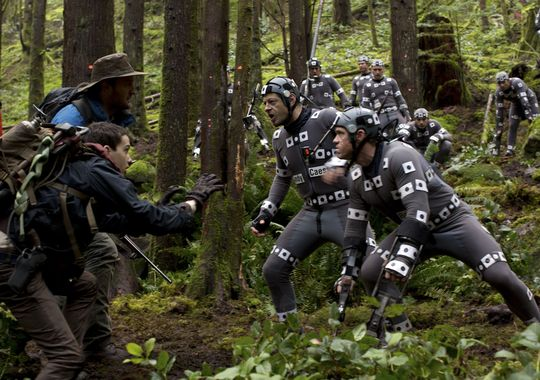
\includegraphics[width=\textwidth]{planet.jpg}
    \caption{Primjer opreme za praćenje pokrena u filmu (preuzeto sa \textit{aeromental.com})}
    \label{planet}
\end{figure}

Kako je već napomenuto ranije u poglavlju, ovakav sustav za praćenje pokreta ima veliki budžetni rang no jeftinije varijante su
vrlo neprecizne i podložne problemima okluzije dok su skuplje varijante suviše skupe ali zato i znatno preciznije. Također problem
je isto i sama infrastruktura i lokacija snimanja jer ovakva postava opreme je vrlo statična i zahtjeva studijske uvjete što si mnoge
ustanove ne mogu priuštiti. Također veliki broj markera za potrebe klasifikacije pokreta nije potreban. Zbog svih ovih problema ovakvo 
rješenje se može iskoristiti no vrlo je skupo i rukovanje ovakvom opremom je često vrlo zahtjevno te je iz tih razloga neadekvatno.

Zadnja razmatrana metoda je ona koja se u ovome radu koristi te ona uključuje korištene inercijskih (IMU) senzora. IMU senzori su
senzori koji se sastoje od akcelerometra, žiroskopa i magnetometra. Korištenjem tih triju informacija moguće je pratiti pokrete u
prostoru. Žiroskop daje informaciju o kutnoj brzini u određenoj osi, akcelerometar daje informaciju o akceleraciji koja djeluje na njega
te magnetometar daje informaciju o magnetnom polju oko sebe koje uz odsustvo bilo kakvih metalnih predmeta i magneta daje informaciju
o orijentaciji senzora u zemljinom magnetnom polju odnosno služi kao svojevrsni kompas. Koristeći sve ove informacije moguće je
pozicionirati uređaj te pratiti pokrete uređaja. IMU senzori se nalaze u svakom pametnom telefonu kao senzor orijentacije kako bi se
prilagodila orijentacija ekrana, zapis o orijentaciji uslikanih fotografija ali i pojedini pametni telefoni kreativnije koriste IMU
senzore te se oni mogu koristiti za upravljanje gestama, primjerice trešnja pametnog telefona pali svjetlo kamere ili
okretanje telefona ekranom prema dole odbija dolazeći poziv i slično. Ovakvi senzori se također koriste za praćenje orijentacije
letjelica u zraku te za mjerenja i nadgledanja vibracija. Oni mogu biti vrlo
malih dimenzija te, kao takvi, mogu biti postavljeni na bilo koje mjesto. Zahtijevaju malo energije za svoj rad stoga se mogu
postaviti na neku udaljenu lokaciju gdje mogu snimati podatke. Cijena takvog senzora je vrlo pristupačna i minimalna cijena trenutno
je 3,33€ od kineskog nabavljača preko stranice AliExpress.com što čini ovakve senzore vrlo povoljnima za nabaviti i koristiti u
većim količinama. Koristeći pseudoperiodičnost ljudskog pokreta proizvođači poput tvrtke Xiaomi su napravili uređaje za praćenje
tjelesne aktivnosti (eng. \textit{Fitness tracker}) u obliku sata koji koristeći IMU senzore mogu detektirati i brojati pojedini korak 
te koristeći BLE (eng. \textit{Bluetooth Low Energy}) šalje telemetriju na pametni telefon na kojemu aplikacija analizira signale
te može prepoznati različite aktivnosti primjerice sjedenje, hodanje, trčanje i slično koristeći samo jedan senzor.

Korištenjem više senzora postavljenih na udovima tijela moguće je puno preciznije snimati kretanja pri čemu osoba ima veliku slobodu,
veću nego u slučaju optičkog praćenja pokreta gdje se slobodno giba ispred kamera, veću nego u slučaju korištenja egzoskeleta u
kojemu sama naprava utječe na kretanje i snima podatke u samo jednoj ravnini te je moguće dobiti više podataka nego što to pružaju
platforme sila. Osoba se može kretati bez prisustva druge osobe te se signali mogu snimati na memorijske kartice ili slati preko
interneta što čini ovakvu metodu prikupljanja podataka vrlo adekvatnom. U daljnjim poglavljima detaljnije se analizira
rad senzora te metode prikupljanja podataka i primjena tih podataka nad neuronskom mrežom kako bi se klasificirali pokreti donjih
ekstremiteta.

\chapter{Analiza IMU senzora}
IMU (eng. \textit{Inertial Measurement Unit}) je elektromehanički uređaj koji služi za mjerenje sila, kutnih brzina te pozicije
uređaja koristeći skup senzora: akcelerometar, žiroskop te magnetometar. Svaki od pojedinih senzora se sastoji od 3 manja senzora
koji svoj posao obavljaju u odnosu na pojedinu os u prostoru. Oni u kombinaciji čine jednu jedinicu koja mjeri vrijednosti u sve 
3 prostorne dimenzije. Rane izvedbe ovakvoga senzora (poput one u Apollo 11 letjelici) su bile vrlo velikih dimenzija i nisu
u sebi imale magnetometar. Danas su se dimenzije IMU senzora znatno smanjile te je moguće izraditi sve potrebne komponente u
sklopu jednog čipa koristeći unaprjeđenja izrade sklopova u samom siliciju. Iako komponente jesu napravljene u siliciju one su
još uvijek elektromehaničke po prirodi što znači da se komponente slobodno gibaju unutar silicijske ploče na samome čipu
te su kao takve mikro-elektromehaničke (skraćeno \textit{MEMS}). Danas su takvi uređaji nezamjenjivi u bilo kakvim letjelicama a
pogotovo u bespilotnim letjelicama (eng. \textit{drone}) koje su u današnje vrijeme sve popularnije. Vrlo su bitni i u
navigacijskim uređajima jer u kombinaciji s GPS uređajima daju dodatnu mogućnost pozicioniranja u slučajevima kada sam GPS signal
nije pristupačan kao što je to, primjerice, u tunelima te dodatno povećavaju preciznost praćenja kretanja. To je jedan od razloga
zašto je IMU senzor neizbježna komponenta pri izradi pametnih telefona. U rukama inženjera, IMU senzori su dobili mnogo raznih 
kreativnih svrha te se mogu naći kao dio kontrolera u igraćim konzolama gdje služe kao dodatna metoda interakcije igrača s igrom.
Prva promatrana komponenta bit će akcelerometar.

\textbf{Akcelerometar}

Akcelerometar je senzor koji mjeri iznos ubrzanja u određenom smjeru. Jednostavan akcelerometar se može koncipirati kao masa ovješena na 
opruzi. Opruga se komprimira onoliko koliko je masa teška, odnosno onoliko koliko je utjecaj gravitacije na tu masu. U slučaju
pojave nove sile u smjeru opruge ona se dodatno otpušta odnosno steže te je ukupan iznos sile na tijelo \textit{"pohranjen"}
unutar opruge, odnosno istog je iznosa, ali suprotne orijentacije. Kako bi se taj iznos mogao očitati u električnome obliku potrebno
je izvršiti pretvorbu a to se može ostvariti na dva načina, koristeći piezoelektrike ili kapacitete. Piezoelektrici
su materijali koji svoju deformaciju mogu pretvoriti u električni impuls te obratno, električni impuls mogu pretvoriti u mehaničku
deformaciju. Vrlo su korisni te njihova primjena varira od senzora koji vibracije akustičnih instrumenata pretvara u električne
signale kako bi se oni mogli snimiti i obraditi, do okidača u džepnim upaljačima koji svojom deformacijom bacaju iskru potrebnu za
započinjanje vatre. Od tog piezoelektričnog materijala se može napraviti opruga te bi kompresija i dekompresija opruge mogla davati
električni signal ekvivalentan iznosu sile na masu. Takva izvedba je vrlo skupa ali vrlo precizna za promatranje nekih pojava,
primjerice visokofrekventnih vibracija.

Druga mogućnost je korištenje kapacitivnosti kao mjeru kompresije i dekompresije opruge. Ako je masa ovješena na opruzi jedna ploča
kondenzatora, onda je površina na kojoj je sama opruga ovješena druga ploča kondenzatora. Ako su te dvije ploče pod naponom,
kompresija i dekompresija opruge približava i udaljava jednu ploču (masu) u odnosu na drugu ploču (površinu) te se kapacitet
povećava, odnosno smanjuje, što opisuje sljedeća jednadžba.

$$
C = \frac{\epsilon A}{d}
$$

U jednadžbi $\epsilon$ predstavlja permitivnost dielektrika koji se nalazi između ploča kondenzatora, $A$ je površina ploča
kondenzatora te je $d$ udaljenost dviju ploča. Površina kondenzatora se ne mijenja, permitivnost je konstantna jer se ne
mijenja dielektrik te jedina promjenjiva varijabla je udaljenost $d$. Načelo rada vidljivo je na slici \ref{accmtr}.


\begin{figure}[h!]
    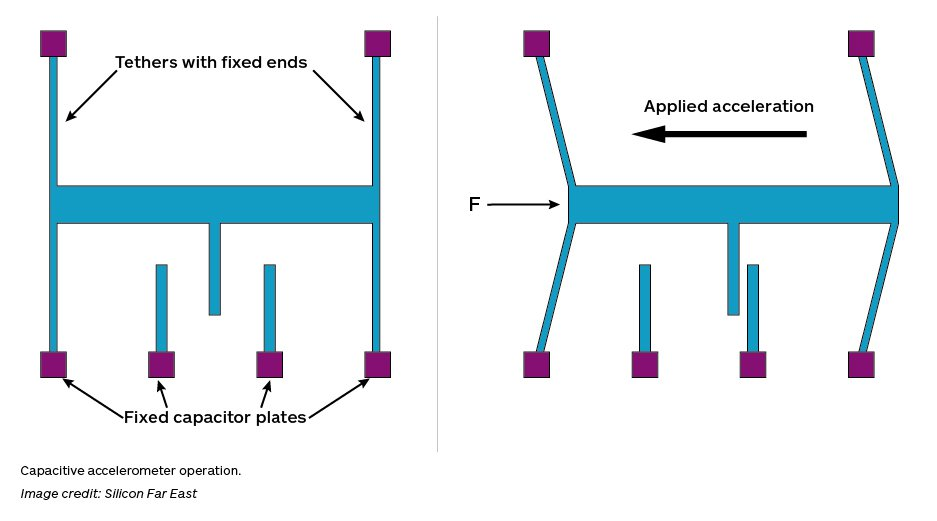
\includegraphics[width=\textwidth]{Accelerometers.jpg}
    \caption{Princip rada kapacitivnog akcelerometra (preuzeto sa \textit{insights.globalspec.com})}
    \label{accmtr}
\end{figure}

Kako bi se dimenzije akcelerometra u potpunosti smanjile, potrebno je razviti takav kapacitivni elektromehanički uređaj napravljen od
silicija koji bi bio u nekom od adekvatnih pakiranja za integrirane krugove. Kako bi bili u mogućnosti promatrati silu u
prostoru potrebno je napraviti pojedini senzor za svaku od tri prostorne koordinate te, kako bi one bile u što većoj mjeri usklađene,
potrebno je sve ostvariti unutar jedne površine silicija kako bi bili skupa unutar integriranoga kruga u fiksnoj poziciji.

\textbf{Žiroskop}

Žiroskop je uređaj koji se sastoji od rotirajućeg diska koji se nalazi unutar kardanskog zgloba (eng. \textit{gimbal}). Rotirajući
disk ima svoju kutnu količinu gibanja koja je promjenjiva jedino onda kada se na rotirajući disk djeluje silom, u protivnom
disk se rotira slobodno u ravnini u kojoj je zavrćen. Kardanski zglob je konstrukcija prstenja koja se oko diska
slobodno može rotirati u svim smjerovima bez da utječe na poziciju diska, odnosno idejno ne djeluje silom na taj disk. Ovakav uređaj
je nezamjenjiv i jedan od najbitnijih komponenti svih letjelica, jer uvijek letjelici daje referentnu točku iz koje se može
zaključiti njen točan položaj u zraku. Koristeći promjenjive otpornike odnosno potenciometre postavljene na osovine kardanskog zgloba,
točna pozicija se može pretvoriti u električni signal koji se dalje može obrađivati i koristiti, primjerice za
automatsku korekciju pozicije bilo kakvog projektila ili letjelice što nudi mogućnost autopilota. Također, kako je brzina prva
derivacija puta u vremenu, tako je i kutna brzina derivacija promjene kuta u vremenu te se iz brzine promjene kuta može izračunati
i kutna brzina prilikom rotacije žiroskopa. Ovakva izvedba žiroskopa je
relativno velikih dimenzija te nikako nije primjerena za ugradnju u uređaje malih dimenzija kao što je to nekakav mobilni uređaj.
Za dizajn uređaja koji je dovoljno malih dimenzija potrebno je opet okrenuti se elektromehaničkim jedinicama implementiranim u poluvodiču.
Kod takve implementacije nije moguće imati rotirajući disk i kardanski zglob što znači da na ovakvoj skali nije moguće ostvariti 
pravi žiroskop koji bi konstantno pratio poziciju uređaja, ali je moguće napraviti uređaj koji mjeri kutnu brzinu.
Takav uređaj se sastoji od vibrirajuće strukture, pojednostavljeno, dvije mase koje titraju istom brzinom u suprotnim smjerovima.
Prilikom rotacije, mase se više ne nalaze u inercijskom sustavu već u akceleriranome što znači da na njih djeluju inercijalne sile.
Kada je sustav u rotaciji unutar njega djeluju razne sile kao što su centrifugalna, centripetalna i Coriolisova sila.
Coriolisova sila je inercijska sila koju tijela doživljavaju prilikom gibanja u rotiranom okviru promatranja. Sveprisutna je na 
planeti Zemlji te je vidljiva prilikom puštanja značajne količine vode u umivaoniku kao smjer vrtloženja vode te je zaslužna za
uragane. Smjer djelovanja Coriolisove sile je okomit na smjer gibanja te na smjer rotacijskog vektora vidljivo na slici \ref{}.

%\begin{figure}[h!]
%    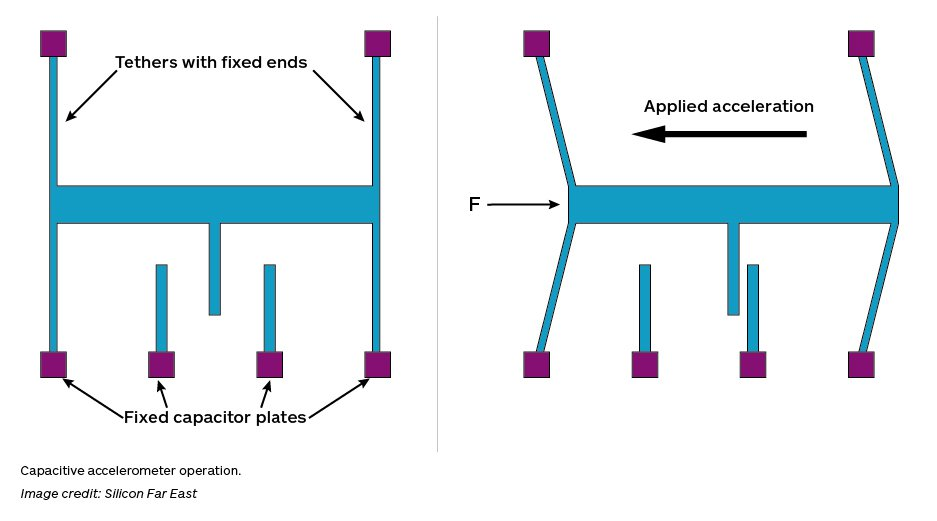
\includegraphics[width=\textwidth]{Accelerometers.jpg}
%    \caption{Princip rada kapacitivnog akselometra (preuzeto sa \textit{insights.globalspec.com})}
%    \label{accmtr}
%\end{figure}

\textbf{Magnetometar}

Magnetometar je senzor koji mjeri jačinu magnetnog polja. Promjena magnetnog polja može
inducirati napon unutar vodiča koji se nalazi u blizini, no na taj se način može detektirati samo promjena. Za mjerenje magnetnog
polja koristi se Hallov efekt. Hallov efekt je fizikalna pojava koja se javlja prilikom gibanja nabijene čestice kroz magnetno polje.
Električki nabijena čestica unutar magnetnog polja mijenja svoju putanju te počinje skretati i u slučaju gibanja po beskonačnoj
površini počinje svoje kružno gibanje pri čemu centripetalnu silu predstavlja Lorenzova sila. Pri ograničenoj površini, nosioc
naboja putuje po vodiču prateći krivulju u smjeru u kojemu na njega djeluje Lorenzova sila te se na taj način istovrsni nosioci
nađu na istoj strani vodiča te nisu nasumično raspršeni po njemu. Ta polarizacija predstavlja napon koji se može izmjeriti pri
čemu iznos tog napona ovisi o kutu između silnica magnetnoga polja i vodiča te samom intenzitetu magnetnoga polja. Kako bi bi se 
nosioci naboja gibali unutar vodiča, potrebno je vodič spojiti na izvor energije, te kako bi oni imali prostora putovati na 
jednu od strana vodiča on mora biti plosnat i veće površine. Primjer načela rada magnetometra vidljiv je na slici \ref{}.

%\begin{figure}[h!]
%    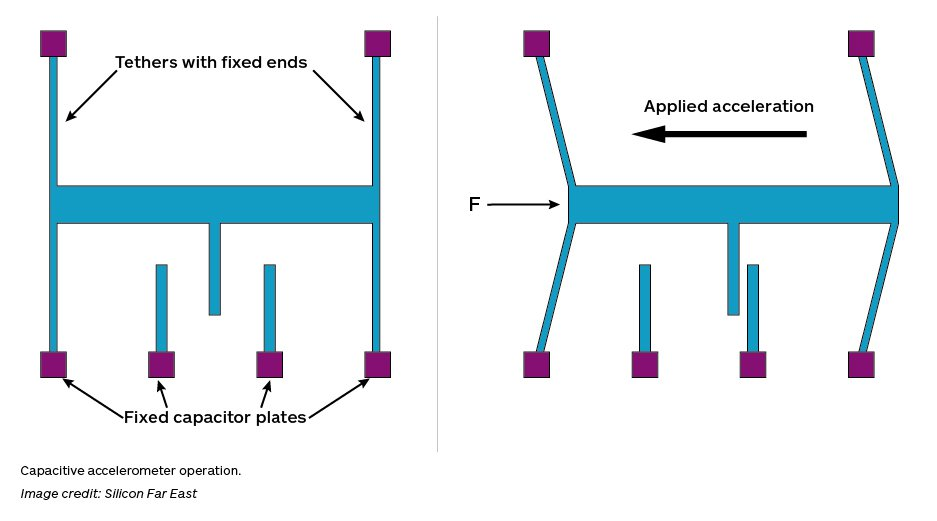
\includegraphics[width=\textwidth]{Accelerometers.jpg}
%    \caption{Princip rada kapacitivnog akselometra (preuzeto sa \textit{insights.globalspec.com})}
%    \label{accmtr}
%\end{figure}

Svaka od opisanih komponenata predstavlja samo dio pojedinog senzora i to dio koji mjeri pojave u samo jednom smjeru. Kako bi se
dobila kompletna slika potrebno je koristiti tri komponente, po jednu za svaki smjer u koordinatnom sustavu. Kako bi se to postiglo
potrebno je osmisliti arhitekturu poluvodičke pločice te paziti na preciznost i ispravno pozicioniranje svake komponente kako bi
ona mjerila točno svoj smjer u odnosu na druge. Ovakvi senzori dolaze često u pakiranju kao pojedini čipovi ili kao jedna cijela
IMU cjelina odnosno SiP (eng. \textit System in Package).

Ovakvih IMU sustava za razvoj uređaja na tržištu ima mnogo. Primjeri su ICM-20948 tvrtke TDK i BMI serija IMU senzora tvrtke
Bosch koji su više industrijski orijentirani. Postoje i oni orijentirani za hobiste i razvoj prototipova primjerice razvojne pločice
tvrtki \textit{Adafruit} i \textit{SparkFun}. Senzor ICM-20948 jedan je od najraširenijih IMU senzora u području znanosti i
industrije iz razloga što zahtjeva vrlo malo snage za rad (2,5 mW) \citep{ICM} što je vrlo poželjno 
za sustave napajane baterijom kao što su to mobilni telefoni ili IoT (eng. \textit{Internet of Things}) uređaji.
Također nudi i digitalni procesor pokreta (eng. \textit{Digital Motion Processor - DMP}) koji služi tome da se algoritmi analize
pokreta mogu izvoditi na tom procesoru čime se rasterećuje glavni procesor ili mikrokontroler što dodatno štedi energiju. Dolazi u
QFN (eng. \textit{Quad Flat No-leads}) pakiranju te je u slučaju nabavke samo takvoga čipa potrebno je izraditi vlastitu tiskanu
pločicu, što je poželjno u slučaju potrebe za nekim prilagođenim rješenjem, no u slučaju izrade prototipa dodaje još jedan zahtjevan
proces u izradi što često nije poželjno. Neke kineske kompanije izrađuju već gotove tiskane pločice koje se mogu nabaviti, što je vrlo
poželjno za izradu prototipa. Druga vrsta takvih senzora su senzori za izradu jednostavnih prototipa i hobiste i primjeri takvih su
Adafruit L3GD20H i SparkFun Razor IMU. Adafruit IMU razvojno okruženje u sebi sadrži čip L3GD20H tvrtke ST te nudi priključke i
pretvarače logičkih naponskih razina kako bi se ova razvojna pločica mogla spojiti sa popularnim razvojnim okruženjima kao što je to Arduino ili
ESP32. Razor IMU sadrži čip MPU-5250 također tvrtke TDK koji je prethodnik već navedenog čipa ICM-20948 te je u trenutku pisanja
ovoga rada označen sa EOL (eng. \textit{End Of Life}) i proizvođač preporučuje korištenje trenutne ICM verzije čipa.
Popularna sučelja kojima se međusobno razvojne platforme i senzori povezuju su I2C i SPI. Bitna razlika između ICM-20948 i L3GD20H
je u logičkim naponskim razinama. ICM za komunikaciju koristi maksimalnih 1,95 V što se bitno razlikuje od naponskih
razina razvojnih okruženja pri čemu Arduino koristi 5V TTL i ESP32 koristi 3.3V TTL. Za korištenje sa takvim okruženjima potrebno je
koristiti most za pretvorbu signala primjerice PCA9306 most za pretvorbu I2C signala korišten u \cite{mini_data_capture}.
Prednost ICM čipa u odnosu na ostale navedene je mogućnost napajanja naponom od 1,8 V pri čemu zahtjeva 3,11 mA struje.
U usporedbi sa L3GD20H kojemu je potrebno 3 V te zahtjeva 5 mA struje, zahtjeva znatno manje snage što je primjerenije za rješenja
koja ovise o baterijskim napajanjima primjerice ugradbeni IoT sustavi ili mobilni telefoni. ICM može koristiti samo pojedine
komponente te svaka od komponenti može podržavati određenu brzinu uzorkovanja. Akcelerometar maksimalno može slati svoja mjerenja
frekvencijom od 4,5 kHz, žiroskop 9 kHz te magnetometar 100 Hz. U dokumentaciji čipa L3GD20H nisu navedene točne frekvencije
uzorkovanja po komponenti, samo su navedene podržane frekvencije između 11,9 Hz i 757,6 Hz. Ove vrijednosti predlažu da je za
potrebu snimanja nekakvih visokofrekventnih vibracija bolji odabir ICM čip, no za potrebe snimanja pokreta djelova tijela visoka
frekvencija nije bitan kriterij. Iz tog razloga valja razmotriti još jednu skupinu IMU senzora, a to su oni koji se nalaze u pametnim
telefonima. Svaki pametni telefon u sebi ima jedan IMU senzor koji tom telefonu daje dodatne funkcionalnosti kao navigaciju, kompas,
rotaciju prikaza ekrana i način upravljanja igrama. Mana ovoga pristupa je ta što sami modeli i specifikacije senzora
nisu javno dostupni podaci, kako bi se došlo do njih potrebno je ili rastavljati uređaje ili potražiti informacije u firmveru.
Iz tog razloga je teže pronaći informacije i tehničku dokumentaciju te saznati neke ključne informacije u slučajevima kada je vrlo 
bitna preciznost i peformansa senzora. Prednost ovoga pristupa je ta što svi mobiteli podržavaju uzorkovanje frekvencijom od 
100 Hz što je prema Nyquistovom teoremu dovoljno za snimanje periodičnih pokreta od gotovo 50 Hz što je i više nego dovoljno za snimanje ljudskih pokreta.
Također ovakav pristup umanjuje e-otpad jer je jedan mobilni telefon već gotov sustav sa vlastitim napajanjem, načinom punjenja,
sučeljem za upravljanje (dodirnik) te mogućnošću spremanja podataka odnosno slanja podataka preko bluetooth veze ili WiFi mreže.
Također, pametni telefoni imaju u sebi vrlo moćne procesore, te bi se na njima mogla i izvoditi sama obrada podataka ukoliko za time
ima potrebe. Kako gotovo svaka osoba posjeduje minimalno jedan takav uređaj, skupljanje podataka u velikoj količini na taj način
postaje vrlo jednostavan i jeftin. Sličan pristup koriste \cite{android} u radu koji koristi samo jedan IMU senzor
postavljen na polovici potkoljenične kosti te uzorkuje signal frekvencijom od 102,4 Hz te putem Bluetooth veze šalje podatke na 
pametni telefon na kojemu se sami podaci obrađuju te je preciznost prepoznavanja pokreta vrlo visoka.

\chapter{Analiza dostupnih baza podataka}
Mnogo je znanstvenih radova napisano na temu ljudskih pokreta i njihovu analizu. Kako bi se ljudski pokreti analizirali, potrebno ih 
je na neki način snimiti, a to se može ostvariti jednom od metoda analiziranih u prijašnjem poglavlju. Kako bi znanost mogla
napredovati te kako bi se drugi ljudi mogli uvjeriti u rezultate rada, mnogi autori svoje podatke stavljaju javno dostupnima.
Ovo će se poglavlje baviti analizom već dostupnih baza podataka, metodom prikupljanja tih podataka, te njihovom svrhom.
Većina dostupnih podataka su prikupljeni podaci o hodu (eng. \textit{gait}). Razlikuju se u broju sudionika, metodi prikupljanja
podataka i svrsi prikupljanja tih podataka.

Prva razmatrana baza podataka je \texttt{whuGAIT} autora \cite{zou2020gait}. U svome radu autori razmatraju mogućnost biometrijske
identifikacije i autentifikacije osoba koristeći specifične karakteristike hoda. Skup podataka sastoji se od podataka prikupljenih
sa pametnog telefona koji se nalazio u džepu snimane osobe pri čemu su se snimali tri osi akcelerometra i tri osi
žiroskopa frekvencijom uzorkovanja od 50 Hz. U prikupljanju podataka je sudjelovalo 118 različitih osoba. Skup podataka je podjeljen
u 8 podskupova od kojih su podskupovi 1-4 namjenjeni za identifikaciju osobe, 5 i 6 za autentifikaciju i skupovi 7 i 8 za
razdvajanje podataka između onih u kojima se vrši hodanje i onih u kojima se ne hoda kako bi se korištenjem neuronske mreže
razdvojio kontinuirani tok podataka. U svim podskupovima su podaci zapisani u tekstualnu datoteku kao CSV vrijednosti. Svaka
tekstualna datoteka predstavlja jednu os akcelerometra odnosno žiroskopa te svaka linija unutar datoteke je uzorak hoda neke osobe.
U posebnoj datoteci se nalaze brojevi koji predstavljaju pojedinu osobu kojoj snimka hoda pripada. Svrha ovih podataka je treniranje
neuronske mreže koja rješava problem n-klasne klasifikacije odnosno pokušava prepoznati i identificirati odnosno autentificirati
osobu bazirano isključivo na njezinom hodu. Koristeći ove podatke \cite{zou2020gait} su dobili preciznost od 93\% u identifikaciji 
i autentifikaciji, no ovi podaci nisu iskoristivi za klasifikaciju pojedinog pokreta jer nisu anotirani za pojedine pokrete te se 
ne može iskoristiti za treniranje takve mreže, no pokazuju da je moguće snimiti vrlo precizne karakteristike pokreta koristeći samo 
jedan pametni telefon.

Sljedeća razmatrana baza podataka je ona koju su snimili \cite{uneven}. Njihov cilj je bio napraviti bazu koja sadrži podatke o
načinu hoda po raznim površinama kako bi uvidili performanse hoda. Prilikom snimanja sudjelovalo je 30 osoba (15 ženskih i
15 muških). Svaka osoba je na sebi imala po 6 IMU senzora: lijeva i desna potkoljenica, lijeva i desna natkoljenica, donji dio leđa
oko L1 kralješka i desno zapešće. Svaka osoba je hodala ravno bez promjene smjera 6 puta po ravnoj asfaltiranoj površini, uzbrdici
odnosno nizbrdici, stepenicama u oba smjera, travnatoj površini, neravnoj kamenoj cigli i šljunku. Podaci svakoga od 6 senzora su
pohranjeni u svojoj CSV datoteci označenoj šifrom iz koje je vidljivo na kojoj se lokaciji nalazio senzor te po kojoj površini
osoba hoda. Podaci svake pojedine osobe se nalaze unutar vlastitog direktorija. Svaki hod unutar direktorija dolazi i sa binarnom
datotekom koja predstavlja te podatke. Uz sve te podatke \cite{uneven} su također obradili i uveli u \textit{Matlab} datoteku pod 
imenom \texttt{data.mat}. Ovakva baza podataka nudi razne mogućnosti poput klasificiranja površine po kojoj osoba hoda ili samo 
detekcija hoda općenito neovisno o površini. Autori su ponudili svoju bazu podataka sa svrhom da unaprijede već postojeće baze
ljudskoga hoda koje su zbog tehničkih ograničenja snimane isključivo u laboratorijskim uvjetima, te kao takve nisu bile primjerene
za analizu primjera iz stvarnoga svijeta. Razvojem IMU tehnologije i bežične komunikacije \cite{uneven} odlučili su napraviti set podataka
snimajući hod u stvarnome svijetu. Ova baza podataka također nije primjerena za potrebe ovoga rada jer su anotirani samo tereni
po kojima ispitanici hodaju te se ne klasificira pokret.

Bazu podataka pod imenom \texttt{HuGaDB} su ostvarili \cite{HuGaDB}. Prilikom provedbe radnji snimljeno je 18 različitih sudionika
koji su snimani sa 6 IMU senzora te 2 EMG senzora. IMU senzori su postavljeni na natkoljenice, podkoljenice te stopala sudionika
pri čemu su snimali radnje: hodanje, trčanje, hodanje uz stepenice, hodanje niz stepenice, samo sjedenje, sjedenje iz stajaćeg položaja,
ustajanje iz sjedećeg položaja, stajanje, voženje bicikla, dizanje unutar dizala, spuštanje unutar dizala i sjedenje
u automobilu kao putnik. Sve radnje su u potpunosti segmentirane što znači da su ispravno anotirane te spremne za treniranje
neuronske mreže. Podaci su pohranjeni u tekstualne datoteke u kojima svaki stupac predstavlja vrijednosti pojedinog segmenta
svakog senzora pri čemu je pozicija senzora označena sa oznakom strane na kojoj se nalazi R i L te pozicijom na nozi F, S i T
(eng. \textit{Foot, Shin i Thigh} redom). Uz poziciju senzora oznaka \textit{acc} i \textit{gyro} označava pojedinu komponentu
IMU senzora te oznake \textit{x, y i z} predstavljaju pojedinu os. Tako jedan segment s oznakom \texttt{acc\_rs\_x} označava
podatke akcelerometra na desnoj potkoljenici u x osi. Svaka tekstualna datoteka se sastoji od identifikatora sudionika,
rednog broja ponavljanja, aktivnosti, verzije i prefiksa koji označava datoteku sa podacima. Tako, primjerice, datoteka sa imenom
\texttt{HGD\_v1\_walking\_17\_02.txt} označava podatke prve verzije baze podataka u kojoj osoba pod rednim brojem 17 hoda po
drugi put. Autori \cite{HuGaDB} na svojoj \textit{github} stranici nude već gotove skripte koje služe učitavanju podataka u
matlab i python programe, te skriptu koja tekstualne datoteke pretvara u \textit{SQLite} bazu podataka.
Ova baza podataka se ne bavi pojedinim djelom tijela, no uzimajući samo podskup 
senzora bilo bi moguće ostvariti prepoznavanje akcije poput vožnje bicikla, hodanja i slično što je onakva klasifikacija pokreta
kakva se razmatra u ovome radu. Problematika ove baze podataka je navedena u uputstvima te navodi da su zbog greške u žiroskopu
neke vrijednosti krive jer je snimak pojačan 10 puta što je dovelo do odsijecanja vrijednosti te je takav signal gotovo neiskoristiv.
Svaki takav slučaj je dokumentiran u tablici te se po potrebi ti podaci mogu izbjeći.

Posljednja razmatrana baza podataka je jedna od najvećih baza podataka hoda s kliničkim anotacijama koju su snimili \cite{pressurePlate}.
Podaci su prikupljani u Austrijskom rehabilitacijskom centru od 2007. do 2018. godine. U prikupljanju je sudjelovalo 2085 pacijenata.
Svaki je pacijent trebao bez ikakvih pomagala prehodati 10 metara preko platformi sila (eng. \textit{Pressure plate}) koje su snimale
GRF (eng. \textit{Ground Reaction Force}) odnosno silu pritiska stopala. Svaki pacijent je svoj hod ponovio 10 puta te je ponavljao
hod na tjednoj bazi. Snimke su anotirane prema dijagnozi te prema razini rehabilitacije kako bi se mogle usporediti i s drugim
pacijentima te kako bi imali uvid u proces rehabilitacije. Problematika ove baze podataka je u tome što se za snimanje pokreta ne
koriste inercijski senzori već se koristi set platformi sila koje snimaju samo silu kojom pacijenti djeluju na njih te takva baza 
podataka nije primjerena za analizu pojedinih pokreta već samo hoda.



\chapter{Stvaranje vlastite baze podataka}
Za stvaranje vlastite baze podataka potrebno je definirati svrhu i ciljeve te baze, a zatim odrediti metodu prikupljanja podataka. U ovome će radu
fokus biti primarno na stvaranje baze podataka korisne za analizu pokreta koja bi se mogla upotrijebiti u svrhe fizikalne terapije koljena.
Za snimanje općenitih pokreta može se iskoristiti mnogo senzora postavljenih po cijelome tijelu, ali za potrebe snimanja jednoga zgloba potrebno je 
koristiti dva senzora, po jedan sa svake strane uda kojeg zglob povezuje. U konkretnom primjeru koljena to su natkoljenica i potkoljenica.

Ovisno o razini preciznosti, cijeni i dostupnosti potrebno je odabrati i same senzore za prikupljanje podataka. Redovito se sustavi senzora
za istraživačke svrhe rade baš za tu namjenu te postoji mnogo sustava otvorenog koda i otvorenih komponenti koji se mogu iskoristiti. Razni
proizvođači nude i svoja komercijalna rješenja za koje garantiraju rad i pružaju podršku ali takvi sustavi ponekad nisu adekvatni za
istraživačke svrhe zbog svoje zatvorenosti i potencijalnog manjka interoperabilnosti s drugim uređajima i programima. U ovome radu, zbog jednostavnosti,
koristiti će se pametni telefon.

Tipičan životni vijek jednog pametnog telefona u prosjeku je dvije godine nakon čega korisnici redovito kupuju nove modele jer stariji postaju neadekvatni
po pitanju trajanja baterije, količine memorije, performansi komponenata i slično. Svaki takav stariji model telefona vrlo često stoji nekorišten iako je još uvijek
funkcionalan. Gotovo svaki pametni telefon u sebi sadrži IMU senzor te u sebi već ima povezivost poput \textit{WiFi i Bluetooth}. Uzimajući u obzir
također da pametni telefoni imaju i ugrađenu bateriju koja može još uvijek biti dovoljno dugotrajna, ekran osjetljiv na dodir kao metodu interakcije i to 
sve ukomponirano u uređaj koji svojim dimenzijama stane u džep, dolazimo do zaključka da su pametni telefoni i više nego adekvatni za prikupljanje podataka.
Također, vrlo je realna pretpostavka da svaka osoba ima pristup minimalno jednome, vjerojatno i dva pametna telefona što čini prikupljanje velike količine
podataka od većeg broja sudionika znatno jednostavnijim. Koristeći držače pametnog telefona za trčanje, uređaji se mogu postaviti osobi na bilo koji
dio tijela na vrlo jednostavan način i svaka bi osoba iz svoga doma mogla pridonijeti stvaranju baze podataka.

Aplikacija koja očitava vrijednosti može biti napravljena posebno, no na tržištu postoje gotove aplikacije, redovito otvorenoga koda, koje se već time bave.
Mnoge aplikacije u trgovini ne nude selekciju samo određenih senzora
već snimaju sve senzore kojima pametni telefon raspolaže te u većini slučajeva nude formatiranu
pohranu podataka isključivo u memoriju uređaja što je vrlo neadekvatno ako bi se uređaji
koristili za obradu informacija u stvarnome vremenu ili za centralizirano prikupljanje podataka na računalo. Neke od takvih aplikacija su
\textit{Sensor Data} i \textit{phyphox} koje se koriste u edukaciji te su u doba COVID pandemije
nezamjenjivi alati za izvođenje fizikalnih eksperimenata kod kuće kao dio
školske zadaće. Nedostatak ovih aplikacija je taj što sve podatke snimaju na lokalnoj memoriji uređaja te nisu primjerene za obradu podataka u stvarnome vremenu.
Aplikacija \textit{Sensorstream IMU+GPS} ne nudi grafičke prikaze podataka već u svojoj vrlo bazičnoj funkcionalnosti nudi odabir senzora uz prikaz trenutnih
vrijednosti istih te odabir akcije koju želimo napraviti s tim podacima. Ponuđene su funkcije spremanja vrijednosti u CSV (\textit{Comma separated value}) formatu,
slanje podataka koristeći UDP protokol te kombinaciju oboje. Za slanje podataka korištenjem UDP protokola potrebno je navesti određenu IP adresu uređaja te \textit{port} na
kojemu uređaj očekuje promet. Također nudi 4 frekvencije uzorkovanja označene sa \textit{slow, medium, fast i fastest}. Te frekvencije uzorkovanja nisu dobro dokumentirane
te nigdje nije navedeno koliko one iznose zapravo. Za mjerenje tih frekvencija može se iskoristiti alat \textit{Wireshark}. Wireshark je alat otvorenoga koda koji
služi za analizu mrežnoga prometa. Vrlo raširen i nezamjenjiv alat za svaku granu računarstva koja se bavi mrežnim prometom. Nudi razne opcije od kojih je jedna 
od moćnijih ugrađeni filter koji vrlo precizno može pronaći određeni paket unutar snimke mrežnog prometa. Koristeći tu mogućnost promet se može snimiti na računalu
te kasnije filtrirati samo one pakete koje mobilni uređaj šalje. Gledajući vremenske indekse prvoga i posljednjega paketa dobivamo ukupno trajanje
snimanja te znajući točan broj paketa može se izračunati približna frekvencija uzorkovanja te su one prikazane u tablici \ref{frekvencije}.

\begin{figure}
    \centering
    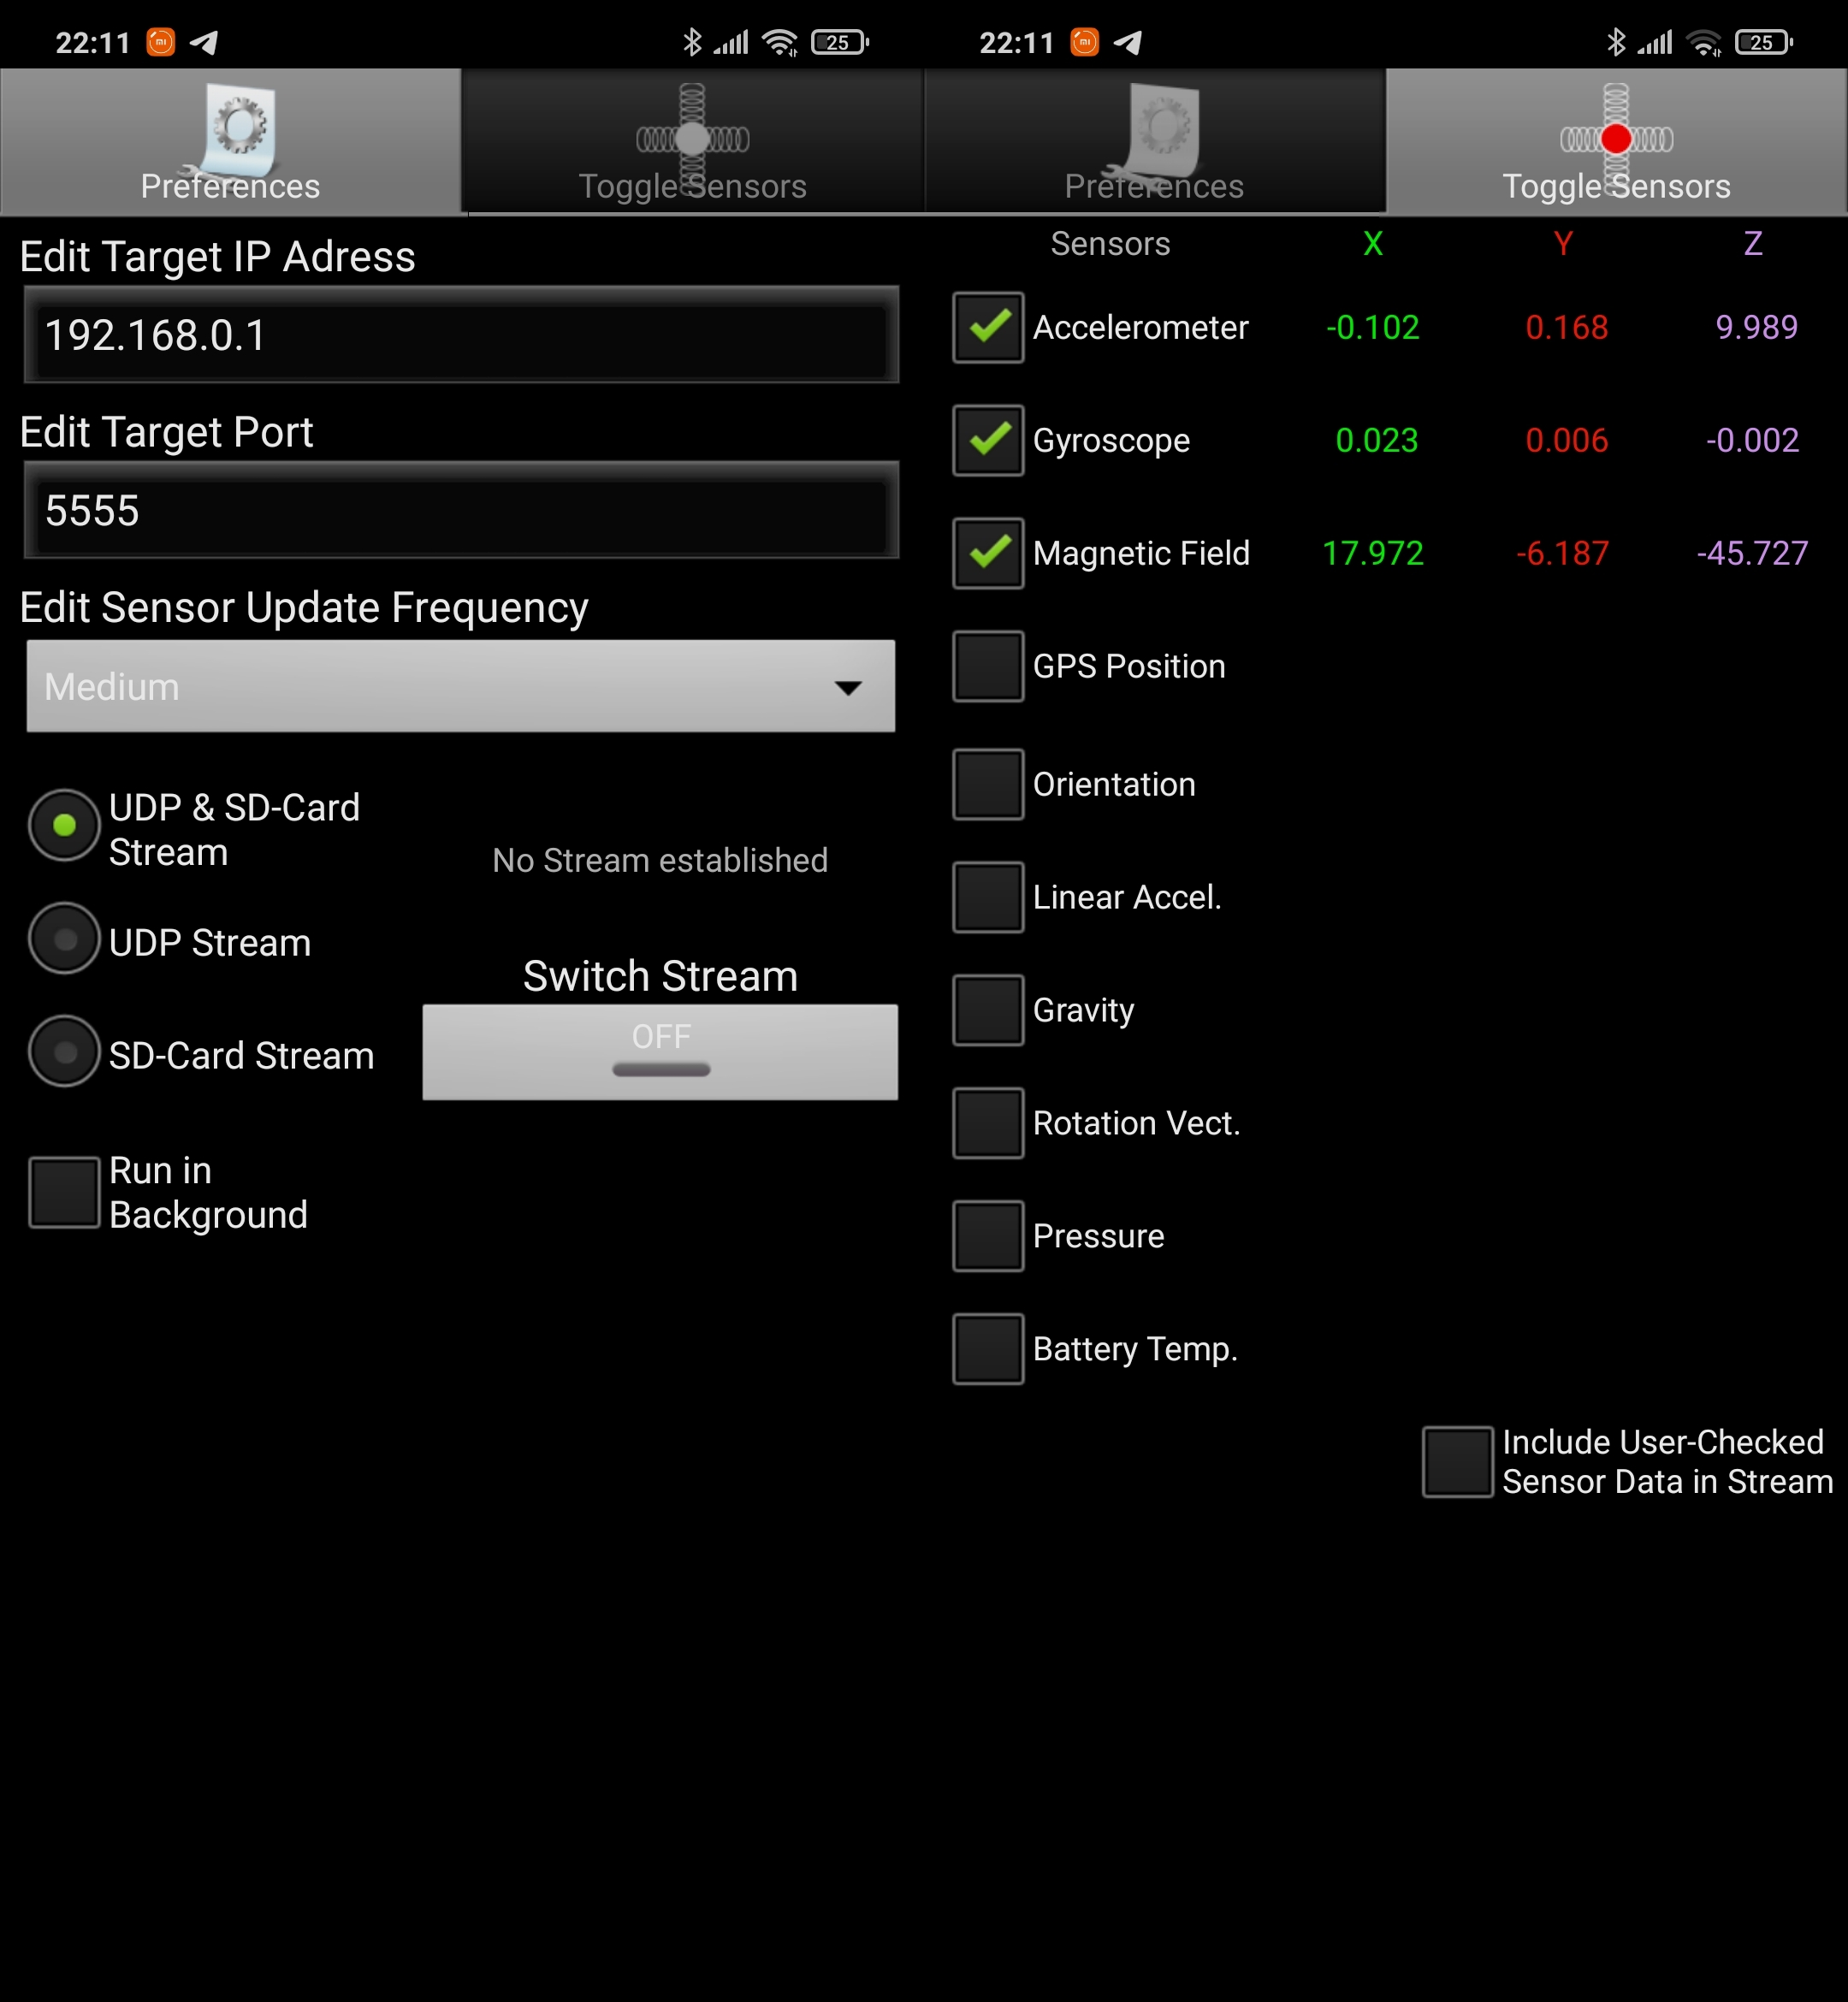
\includegraphics[width=250px]{app.jpg}
    \caption{Izgled aplikacije Sensorstream IMU+GPS}
\end{figure}

\begin{table} [h!]
 \centering
    \begin{tabular}{|c|c|c|c|}
        \hline
        Uzorkovanje & Trajanje (s) & Broj poruka & Frekvencija \\
        \hline
        Slow & 12.21 & 61 & 5 \\
        Medium & 3.98 & 61 & 15 \\
        Fast & 6.85 & 344 & 50 \\
        Fastest & 2.14 & 299 & 124\\
        \hline
    \end{tabular}
    \caption{Izmjerene frekvencije uzorkovanja}
    \label{frekvencije}
\end{table}

Također, koristeći Wireshark alat može se jedan paket analizirati i vidjeti format podataka koju uređaj šalje. Podaci su u CSV formatu u kojima se šalje vremenski indeks,
identifikacijski brojevi senzora te same vrijednosti senzora kako se vidi u slici \ref{datagram}. Svi podaci prikazuju vrijednosti redom $x$, $y$, i $z$ osi.

\begin{figure}[h]
    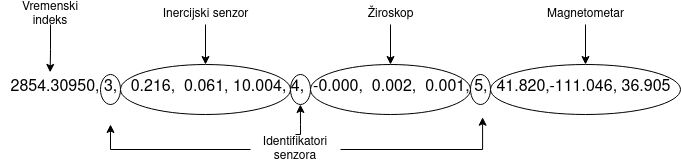
\includegraphics[width=\textwidth]{datagram.png}
    \caption{Primjerak primljenih podataka}
    \label{datagram}
\end{figure}

Kako bi se ti podaci primili i pohranili na adekvatan način potrebno je napraviti program klijent koji osluškuje na određenim portovima. Implementacija tog programa 
u ovome radu biti će napravljena koristeći skriptni jezik python. 

Python je vrlo popularan jezik mnogih mogućnosti koji je vrlo jednostavan za učenje i korištenje te zbog svoje popularnosti raspolaže mnogim bibliotekama.
Neke od tih vrlo korisnih biblioteka koje će biti korištene u ovome radu su \textit{NumPy}, \textit{Matplotlib} te \textit{socket}. Python se kao skriptni jezik
izvodi liniju po liniju te se svaka linija interpretira tek kad ona dođe na red za izvršavanje što ukida proces prevođenja programa u strojni kod kao što je to primjerice
potrebno kod programskog jezika \textit{C}. Iz tog razloga je vrijeme izvršavanja takvoga koda znatno dulje što utječe na performanse programa. Kako bi se
izvođenje kompliciranijih matematičkih operacija znatno ubrzalo te kako bi se ponudio veći opseg već gotovih funkcija napravljena je biblioteka \textit{NumPy}.
NumPy je biblioteka koja nudi gotovo sve potrebne funkcije za izradu programa koji se koriste u znanosti. Implementira višedimenzionalne matrice te sve funkcije
za operaciju nad njima uključujući promjenu oblika matrice, konkatenacije matrica te sve ostale matrične operacije. Također nudi i funkcije za Fourierovu transformaciju, statističku obradu,
generatore nasumičnih brojeva i slično. NumPy implementacija matrica je znatno bliža onakvim matricama kao što su u programskome jeziku C te su kao takve memorijski
znatno manje zahtjevne od originalnih matrica koje nudi python. Također kako bi operacije nad matricama bile brze operacije su implementirane u programskome jeziku C te
prevedene unaprijed tako da biblioteka nudi vrlo jednostavnu sintaksu uz jako veliku brzinu izvođenja te manju veličinu datoteke pri pohrani podataka.
Biblioteka \textit{socket} nudi funkcije za umreživanje koje su potrebne kako bi se podaci uspješno primili s mobilnih uređaja je \textit{Matplotlib} koji je potreban
za vizualizaciju podataka u obliku grafova.

\begin{lstlisting}[caption=Ostvarivanje veze na strani klijenta, label=socket]
def init_client(srv_port):
    client_socket = socket.socket(family=socket.AF_INET,\\
                                    type=socket.SOCK_DGRAM)
    client_socket.bind((self_ip, srv_port))
    return client_socket

client = []

client.append(init_client(port))
print("UDP client up") 
\end{lstlisting}

U kodu \ref{socket} je vidljiv način na koji se koristi biblioteka \textit{socket}. Svaki mobilni uređaj predstavlja instancu klase \textit{socket} koju se sprema
u listu klijenata \texttt{client} što omogućuje povezivanje proizvoljnog broja mobilnih senzora, pri čemu svaki senzor treba imati svoj poseban port. Port na računalu
bi trebao biti slobodan odnosno niti jedna druga aplikacija ne bi smjela koristiti taj port za svoj promet. Dobra praksa nalaže da se za osobne potrebe koriste portovi
brojeva većih od 1024 kako bi se izbjegli mogući zauzeti portovi nekakvih standardnih protokola kao što su \textit{https} i slični. U ovome slučaju mobilni uređaj
s indeksom 0 koristi port broja 5555 te svaki sljedeći zauzima port $5555 + i$ pri čemu je $i$ indeks uređaja. Točan broj je potrebno unijeti ručno na svaki uređaj
koji šalje podatke. Stvaranje instance \textit{socket} odvija se u liniji 2 i 3 pri čemu se u argumentu treba navesti tip veze. Za familiju veze se navodi
\texttt{AF\_INET} što predstavlja IP protokol te pod tip se navodi \texttt{SCOK\_DGRAM} što označava korištenje UDP protokola. UDP (eng. \textit{User Datagram Protocol})
je jedan od osnovnih transportnih protokola koji podatke prenosi po principu \textit{best effort}, pretpostavlja se da su datagrami došli do odredišta u ispravnome redoslijedu
te se ne potvrđuje primitak datagrama. Ovakav protokol ne garantira cjelovitost podataka, no nudi manje zagušenje prometa zbog nedostatka potvrđivanja svakog primljenog
datagrama i retransmisije u slučaju gubitka te se iz tog razloga koristi za prijenos videa i VoIP (eng. \textit{Voice over IP}) pozive. U liniji 4 se instanca razreda
\textit{socket} povezuje s odgovarajućim portom na odgovarajućem mrežnom uređaju koji je predstavljen vlastitom IP adresom \texttt{self\_ip}. Na kraju funkcija
\texttt{init\_client} vraća instancu kako bi bila spremljena u klijentsku listu.

\begin{lstlisting}[caption=Primanje podataka, label=primanje]
while(True):
    sample = []
    for phone in client:
        bytes_adress_pair = phone.recvfrom(buffer)
        data = []
        message = bytes_adress_pair[0].decode().split(",")
        for i in message:
            data.append(i.strip())

        # filteri podataka
        if "4" not in data:
            continue

        for i in data_filter:
            data.pop(i)
        
        if len(data) != 0:
            sample.append(data[:6])
            
    if len(sample) != 0:
        signal.append(sample)
    else:
        continue
\end{lstlisting}

U odsječku koda \ref{primanje} prima se datagram svakog mobilnog uređaja. Svaki datagram se uzima iz međuspremnika koji je veličine 1024 bajta. Svaki datagram se sastoji
od samih podataka (u 6. liniji koda pod indeksom 0) te IP adrese pošiljatelja koja u ovoj implementaciji nije potrebna te se može izostaviti. Nad podacima se vrše obrade
poput uklanjanja praznina (linija 8.) te rastavljanje podataka iz jednog monolitnog zapisa podataka u više zasebnih podataka pomoću \texttt{split} funkcije uzimajući
zarez kao graničnik. Zatim te podatke valja filtrirati pri čemu se uklanja \textit{vremenski indeks}, identifikatori senzora te podaci magnetometra
prikazanih na slici \ref{datagram}. Eksperimentalno se pokazalo da se pri prvih nekoliko mjerenja od početka slanja podataka sa mobilnih uređaja izostavljaju vrijednosti
žiroskopa te se gledajući prisutnost tih vrijednosti dodatno vrši čekanje na spremnost svih senzora u mobilnome uređaju. U ovome kodu to se vrši uvjetovanjem u liniji 11.
Struktura podataka je prikazana u slici \ref{struktura}.

\begin{figure}[h]
    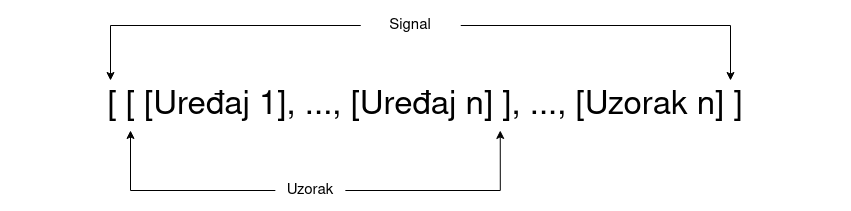
\includegraphics[width=\textwidth]{OrganizacijaPOdataka.png}
    \caption{Struktura podataka}
    \label{struktura}
\end{figure}

Uzorak jednoga uređaja je lista vrijednosti njegovih senzora. Jedan uzorak je lista uzoraka \textbf{svih} uređaja. Signal je samo lista uzoraka. Na ovaj se način akcija 
može snimiti i koristeći biblioteku \textit{NumPy} pohraniti na računalo za daljnju obradu.

Kako bi se prikupili odgovarajući podaci za treniranje i uporabu neuronske mreže potrebno je iz toka podataka izdvojiti pojedina ponavljanja vježbi kako bi samo ti bitni
segmenti ili bili prikupljeni za treniranje neuronske mreže ili kako bi se pojedini segment predao neuronskoj mreži na klasifikaciju. 
Mnogi radovi primjerice \cite{android}, \cite{exo} i \cite{LowerLimb} spominju pronalazak karakterističnih točaka unutar signala
kao jednu od glavnih faza predobrade signala. Ovisno o željenom rezultatu moguće je promatrati statičke osobine signala
kao što su to prosjek, standardna devijacija, varijancija i slično te dinamičke kao što su to energija, prosjek energije, odnos
harmonika, energetska entropija i slično \citep{android}. Također je moguće napraviti posebne klasifikatore koji su, u suštini,
neuronske mreže trenirane posebno za detekciju pojedinih osobina signala kao što su to napravili \cite{exo}. 
Najjednostavniji pristup tome je promatranje samo jedne osi određenoga senzora u nekome vremenskom periodu kao što su to napravili
\cite{LowerLimb}. Promatranjem samo jedne osi jednoga senzora fokus može biti na pseudoperiodičnosti tog signala te se detekcija
periodičnosti i segmentacija može odviti pomoću detekcije rubnih vrijednosti. Izvođenjem jednostavnije vježbe poput ekstenzije
potkoljenice (eng. \textit{leg extension}) s obzirom na poziciju mobilnog uređaja koji se nalazi ekranom okrenutim od potkoljenice uspravno na
potkoljenici može se sav fokus staviti na vrijednosti žiroskopa u $x$ osi. Snimajući te iscrtavajući odgovarajuće vrijednosti
na grafu jasno je vidljiv period te same karakteristike funkcije (slika \ref{period}). Dok se vježba ne izvodi signal je
vrlo miran i iznosi približno 0. U trenutku početka pružanja potkoljenice zbog smjera rotacije mobilnog uređaja kutna brzina iznosi
otprilike $-2,5 rad/s$. Zatim se potkoljenica u stanju potpune ispruženosti smiri te kutna brzina iznosi 0. Pri spuštanju kutna
brzina raste te također iznosi približno $2,5 rad/s$, ali u ovom slučaju u pozitivnom smjeru. Uzevši ove vrijednosti može se ostvariti
konačan automat koji prati vrijednosti signala te mijenja stanja u odnosu na iste pri čemu se pamti početak perioda. Ako se automat nađe u
prihvatljivom stanju onda to predstavlja kraj periode te je poznat cijeli segment signala koji predstavlja jedno ponavljanje.
Ovakav signal se pohrani te se čeka nova perioda. U slučaju da ponavljanje nije dobro, odnosno da iz nekog razloga
karakteristične vrijednosti nisu dosegnute zbog krivog izvođenja ili je osoba ne izvodeći vježbu slučajno
dosegla vrijednost okidanja zbog kojeg je automat ostao u krivome stanju, potrebno je vremenski ograničiti
izvođenje vježbe. Ako osoba ne izvede vježbu unutar nekog određenog vremena koje ovisi o vježbi automat se vraća
u početno stanje te se čeka novi period.

\begin{figure}[h!]
    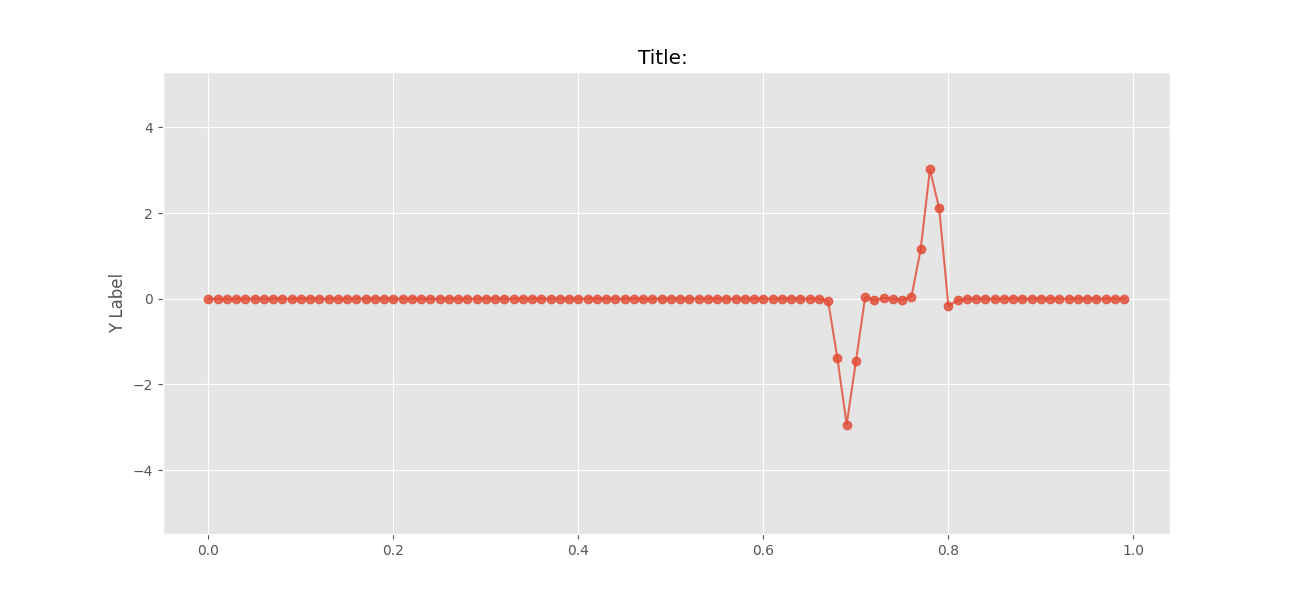
\includegraphics[width=\textwidth]{period.png}
    \caption{Primjer jednog ponavljanja vježbe, x - vrijeme, y - kutna brzina}
    \label{period}
\end{figure}

Anotacija signala može biti izvedena na više načina. Podaci mogu biti pohranjeni u pojedinim datotekama kojima
se anotacija nalazi u nazivu kao što je to kod \cite{HuGaDB}. Ovakav pristup omogućuje da se anotacija vrlo
lako programski može učitati prilikom učitavanja relevantnih podataka iz datoteke no za to je potrebno ručno
imenovati datoteku prilikom svakog snimanja podataka. Podaci mogu biti anotirani u posebnoj datoteci koja se
nalazi skupa sa samim podacima kao što je to u \cite{zou2020gait} gdje su podaci pohranjeni u svom direktoriju
dok je datoteka s anotacijom izvan tog direktorija. Također moguće je i pohraniti anotaciju unutar datoteke s
podacima, no radi praktičnosti učitavanja podataka znatno je jednostavnije imati anotacije izvedene na jedan od
navedenih načina. Podaci se također mogu pohraniti na više načina. Za korištenje sa NumPy bibliotekom moguće je
podatke jednostavno pohraniti u obliku matrice u binarnoj \texttt{.npy} datoteci no ovakva datoteka nije čitljiva
koristeći druge programske biblioteke i pakete. Postoji mogućnost da je neka interoperabilnost implementirana
sa bibliotekama u drugim programskim jezicima zbog popularnosti NumPy biblioteke, no to nije dobra praksa.
Najveću interoperabilnost se može postići koristeći jedan od otvorenih i čestih formata
kao što je to obična tekstualna datoteka u kojoj su vrijednosti zapisane u ljudski čitkom ASCII formatu,
CSV zapis, JSON i XML (iako su zadnja dva formata za potrebe pohrane signala neadekvatni).
Na ovaj način, neovisno o odabranoj tehnologiji, podaci se mogu na jednostavan način učitati i za potrebe bržeg
pristupa podataka pohraniti u binarnom obliku po izboru. Dokle god su podaci u nekom obliku koji se može lako
učitati, sam način zapisa nije toliko bitan, ono što je uz set podataka najbitnije je dobra dokumentacija koja
opisuje točnu strukturu, oblik i format podataka. Za popularne formate podataka kao što su to CSV podaci, nije toliko
krucijalno jer su često podaci unutar datoteke već opisani te postoje već gotove funkcije za učitavanje takvih
podataka u gotovo svakom programskom jeziku. Dokumentacija je bitna kad se podaci zapisuju u tekstualnu datoteku
jer iz samih podataka često nije jasan njihov format odnosno što predstavlja redak a što stupac.
\cite{HuGaDB} su uz posebnu \texttt{README} datoteku u svaku datoteku upisali i zaglavlje u koje su zapisani
metapodaci kao što su ime aktivnosti odnosno dodatna anotacija podataka, datum snimanja te su označeni stupci
u kojima se nalaze podaci. Za učitavanje podataka je također dobra praksa i vrlo korisno svima koji će tu bazu
podataka koristiti ustupiti vrlo jednostavne elementarne programe implementirane u raznim programskim jezicima
koji učitavaju podatke na ispravan način kako bi korisnik taj kod jednostavno mogao uključiti u vlastiti kod i
koristiti već gotovu funkciju. Primjer takvog koda je prikazan u isječku \ref{load}.

\begin{lstlisting}[caption=Funkcija za učitavanje HuGaDB podataka, label=load]
    def load_file(path_to_file):
        return np.genfromtxt(path_to_file, delimiter='\t', \\
                                skip_header=4, \\
                                dtype=np.float32)
\end{lstlisting}

Ovo je primjerak enkapsulacije već gotove NumPy funkcije koja iz formatirane tekstualne datoteke učitava vrijednosti s 
postavkama pomoću kojih te podatke učitavaju na ispravan način. Ovu funkciju su za svoj set podataka napisali \cite{HuGaDB}.
Funkcija kao argument prima apsolutnu putanju do
datoteke te vraća objekt tipa \texttt{numpy.array}. Ostali argumenti govore funkciji da su podaci tipa
float veličine 32 bita, da postoji zaglavlje od 4 redaka koje nije dio podataka te da su svi podaci razdvojeni
tabulatorom.

\chapter{Implementacija metode strojnoga učenja}
Strojno učenje (eng. \textit{Machine learning}) je znanost o algoritmima koji se korištenjem podataka vremenom
automatski poboljšavaju. Ti algoritmi imaju dvije svrhe, predviđanje budućih događaja i klasifikaciju podataka
s obzirom na podatke kojima je izgrađen model. Za ostvarenje svrha tih algoritama potrebne su dvije ključne
stvari, neuronska mreža i skup podataka. Neuronska mreža je, u računalnom smislu, mreža umjetnih neurona koji su
međusobno povezani između slojeva te svojim radom imitiraju biološke neurone. Jednostavan neuron sastoji se
od svojih ulaza, izlaza neurona iz sloja prije na koje je primjenjena neka težina te izlaza. Jednostavan
neuron sumira vrijednosti prijašnjih neurona sa težinom te tu vrijednost normalizira i kao takvu ju šalje
u sljedeći sloj koji radi isti takav postupak. Normalizacija vrijednosti je postupak kojim se vrijednosti
unutar mreže održavaju na nekoj maloj razini, često između 0 i 1 ili između -1 i 1 kako vrijednosti u mreži
ne bi dosezale velike iznose. To se ostvaruje korištenjem aktivacijske funkcije u neuronu a takva funkcija može
biti primjerice $tanh$, $sig$ ili najjednostavnija $step$ funkcija. Svaka se mreža sastoji od tri glavna sloja,
ulazni sloj, skriveni sloj i izlazni sloj. Ulazni i izlazni slojevi imaju onoliko neurona koliko ima samih
ulaza odnosno izlaza. U skrivenome sloju se može nalaziti proizvoljan broj slojeva od kojih svaki sloj ima
proizvoljan broj neurona. U klasičnome slučaju neuroni su jednosmjerni te se tok podataka odvija iz sloja u
sloj od ulaza prema izlazu, no danas postoje razne mreže koje ne prate klasičan model. Kako bi se vrijednosti
težina između neurona ugodile tako da mreža izvodi željenu funkciju, potrebno je provesti treniranje mreže
koristeći set podataka koji predstavljaju primjere točnih ulaza i izlaza funkcije. Za bolje rezultate treniranja
potrebno je imati što je više moguće kvalitetnih podataka koji što vjernije predstavljaju realne probleme i
rješenja kakvi bi se našli u stvarnoj primjeni. Za to je potrebno na korektan način prikupiti što veći broj
podataka. Primjeri takvih podataka se mogu naći na internetu, neki od primjera su IMDB skup podataka za 
prepoznavanje mišljenja u kojemu su podaci binarno anotirani odnosno svaka kritika je anotirana kao dobra ili
loša. Nakon treniranja, mreža je u mogučnosti zaključiti iz teksta nalazi li se u njemu dobra ili loša kritika.
Još jedan primjer podataka je MINST baza podataka koja se sastoji od 60000 slika od 25x25 piksela
rukom pisanih znamenki te oznakama koje se znamenke na tim slikama nalaze. Nakon treniranja mreža je sposobna
na slici prepoznati rukom pisane pojedine znamenke. Prilikom učenja mreža svakog koraka, koristeći trenutne
vrijednosti težina veza koje u početku mogu biti nasumične, na izlazu aktivira neuron za koji trenutno misli
da bi trebao biti upaljen. Ta se vrijednost uspoređuje sa traženom iznaznom vrijednosti te se između tih dviju
vrijednosti računa pogreška (eng. \textit{loss}). Ta pogreška se koristi za ugađanje težina veza između neurona
koristeći neku od metoda prostiranja podataka unazad (eng. \textit{backpropagation}) kao što je to gradijentni
spust te se ponovno koriste podaci iz skupa podataka za treniranje kako bi se opet izračunala pogreška
odnosno mreža ulazi u novu epohu.
Pogreška nikada neće iznostiti nula no može biti dovoljno mala. Nakon faze treniranja mreže, uz uvjet da su
rezultati zadovoljavajući, ona se može koristiti nad realnim podacima uz određenu vjerojatnost pogreške koja
je često vrlo mala. Točnost mreže se može izraziti kao omjer pogođenih izlaza i svih izlaza, no ova vrijednost
nije vrlo mjerodavna kada se mjeri nad skupom podataka kojima je mreža bila trenirana. Može biti dobar indikator
do koje mjere je mreža točna no u slučaju prekomjernog učenja mreže ona "zapamti" parove vrijednosti iz skupa
za treniranje što daje dojam da je mreža vrlo precizna, no pri analizi koristeći druge podatake ona daje loše rezultate.
Ova pojava se zove pretreniranost (eng. \textit{overfitting}). Kako bi se ona detektirala potrebno je imati
testni skup podataka koji nikako ne sudjeluju u samom treniranju mreže. Ti podaci služe tome da se nakon treniranja
mreža validira nad podacima koje do sada "nije vidjela" odnosno nije mogla zapamtiti
te ovakvi podaci daju bolji dojam o točnosti mreže. Obično ti testni skupovi podataka nisu posebni skupovi već
se iz skupa svih podataka izdvoji jedan udio koji služi svrsi testiranja. Ovaj korak je krucijalan i
ne smije se izostaviti. Za izbjegavanje pretreniranosti mreže podatke je potrebno na neki način nasumično
pomiješati odnosno pobrinuti se o tome da prilikom treniranja na ulaz mreže ne dolaze sekvecijalno istovrsni
podaci jer će to loše utjecati na cijelokupan ishod. Na primjer, ako se vrši analiza slike na kojoj bi mreža
trebala prepoznati psa ili mačku, u slučaju da prvih $n$ podataka predstavlja psa na slici mreža bi radila odlično
kod prepoznavanja pasa, no ne bi bila dobra pri prepoznavanju mačaka ili bi u ekstremnom slučaju mislila da se
na svim slikama nalazi pas. Također je vrlo bitno da skup bude što raznolikiji jer u slučaju male raznolikosti
mreža također ne bi radila očekivano što bi se u istoj analogiji prepoznavanja ljubimaca na slici moglo
manifestirati na način da prepoznaje samo jednu vrstu psa odnosno mačke ili prepoznaje samo u slikama koje su
slikane iz određenog kuta. Podaci moraju biti što raznovrsniji iz razloga što se zahtjeva od mreže da radi u
nekom općem slučaju.

Kako se neuronske mreže koriste nad raznim različitim podacima postoji mnogo arhitektura i vrsta mreže no za
ovaj rad je najbitnija RNN (eng \textit{Recurrent Neural Network}). RNN mreža je mreža koja u sebi sadrži
sloj neurona koji imaju povratnu vezu. Povratna veza u neuronu služi kao kao unutarnja memorija te je iz tog razloga
vrlo povoljna za analizu toka podataka kao što su signali u vremenu ili pisani tekst u kojemu je bitno imati informaciju
o tome što se ranije našlo na ulazu. Danas se za to koriste LSTM (eng. \textit{Long Short-Term Memory}) ćelije.
LSTM ćelije su ćelije sa povratnom vezom koje se sastoje od više segmenata odnosno vrata. Povratnom vezom
je ostvarena unutarnja memorija koja ulazi u vrata zaborava. Također u vrata zaborava ulaze i sam ulaz te
izlaz LSTM ćelije iz sloja prije. Ulaz podataka i informacija prijašnje ćelije se vektorski kombiniraju te
se normalizacijom vektora koristeći sigmoid funkciju dobiva vektor zaborava s vrijednostima između 0 i 1.
Matrično se množi s trenutnom unutarnjom memorijom pri čemu elementi pomnoženi s brojevima bliskim nuli
iščezavaju, odnosno oni se "zaboravljaju". U ulazna vrata ulazi ista kombinacija ulaza kao i u vrata zaborava
pri čemu se oni dijele u segment koji se normalizira sigmoid funkcijom i segment koji se normalizira $tanh$
funkcijom. Tangens hiperbolički služi isključivo normalizaciji podataka te matrično pomnožen sa segmentom
iz sigmoid funkcije opet odlučuje koji segmenti su više bitni, a koji nisu te se dodaju unutarnjoj memoriji
za sljedeći korak. Na kraju u izlazna vrata ulazi novo stanje unutarnje memorije normaliziran funkcijom
$tanh$ te sigmoid ulaznih podataka. Njihov matrični umnožak predstavlja izlaz iz LSTM ćelije te taj podatak
ulazi u ulaz sljedeće ćelije skupa sa ulaznim podatkom. LSTM ćelija je prikazana na slici \ref{lstm}.
Ovakve ćelije su potrebne zbog problema pri rasprostiranju unatrag. Naime koristeći gradijentni spust sam
gradijent svakim slojem iščezava te u većini slučajeva prvi slojevi u RNN mreži nisu na nikakav način korigirani
prilikom učenja što znatno utječe na performanse mreže. Koristeći LSTM ćelije gradijent ne iščezava te
se težine ispravno ugađaju.

\begin{figure}[h!]
    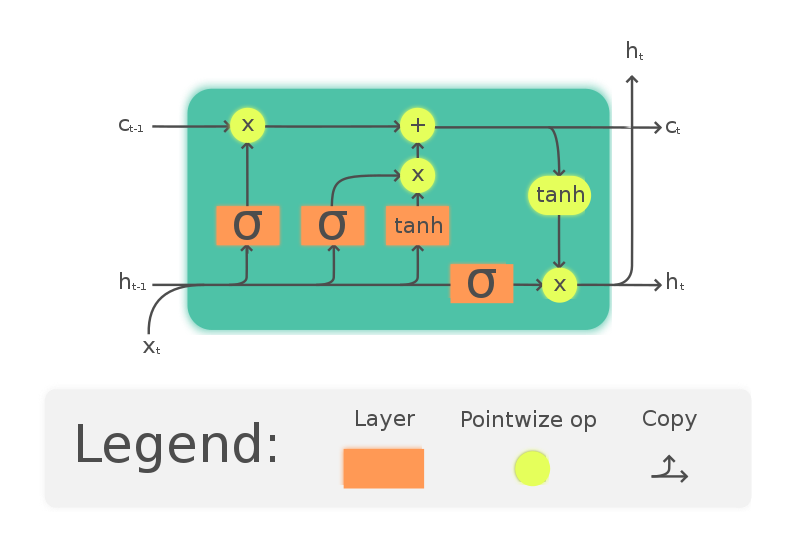
\includegraphics[width=\textwidth]{The_LSTM_Cell.svg.png}
    \caption{Logički prikaz jedne LSTM ćelije (preuzeto sa \textit{wikipedia.com})}
    \label{lstm}
\end{figure}

U ovom radu će se za izradu neuronske mreže koristiti Keras. Keras je sučelje za TensorFlow napisano u programskom jeziku
python koje služi za brzu i jednostavnu izradu modela neuronskih mreža.
TensorFlow je jedna od najpopularnijih platformi za strojno učenje. Otvorenoga je koda te njegove biblioteke
nude gotovo sve funkcije potrebne za primjenu strojnoga učenja. Keras kao sučelje nudi vrlo visoku razinu
apstrakcije u izradi neuronskih mreža te je uzevši u obzir doseg ovoga rada dobar izbor za implementaciju.

Ostvarena mreža se uvelike bazira na mreži korištenoj u primjerima obrade ranije spomenute analize rukom
pisanih znamenki. U tom primjeru se rješava problem n-klasifikacije pri čemu postoji 25 ulaza u mrežu od kojih
svaki predstavlja jedan redak od 25 piksela. Prolaskom kroz mrežu aktivira se jedan od 10 izlaznih neurona
koji predstavlja jednu znamenku od 0 do 9. U ovome radu će se obrađivati HuGaDB baza podataka opisana u ranijem
poglavlju. Od svih dostupnih podataka koristit će se podskup senzora kakav je opisan u poglavlju ranije odnosno
akcelerometri i žiroskopi koji se nalaze postavljeni na podkoljenici i nadkoljenici desne noge. Kako ti senzori
predstavljaju ukupno 12 istovremenih signala, ulaz u mrežu treba biti veličine 12. Kako je skup podataka anotiran
za akcije opisane u ranijem poglavlju, potrebno je izdvojiti skup podataka za testiranje od skupa podataka za 
treniranje što je bilo napravljeno manualnim nasumičnim odabirom nekolicine primjera svakog kretanja. Zbog malog broja
primjera nekih pokreta kao što su putovanje liftom i hodanje po stepenicama neki podaci su zanemareni te se 
razmatra samo 6 kretnji: vožnja bicikla, trčanje, sjedenje u automobilu, statično sjedenje, stajanje i hodanje.
Iz tog raloga izlaz treba biti veličine 6. Zbog jednostavnosti Keras sučelja sama implementacija mreže je
vrlo kratka i jednostavna. Slijedi kod koji implementira mrežu.

\begin{lstlisting}
    import numpy as np
    import tensorflow as tf
    from tensorflow.keras.models import Sequential
    from tensorflow.keras.layers import Dense, Dropout, LSTM
    import tensorflow.keras.optimizers

    final_len = 5300
    
    x_train = np.load("x_train_normal.npy")
    y_train = np.load("y_train_normal.npy")
    x_test = np.load("x_test_normal.npy")
    y_test = np.load("y_test_normal.npy")
    
    model = Sequential()
    model.add(LSTM(128, input_shape=(12, final_len), \\
                activation='relu', return_sequences=True))
    model.add(Dropout(0.2))
    
    model.add(LSTM(128, activation='relu'))
    model.add(Dropout(0.2))
    
    model.add(Dense(32, activation='relu'))
    model.add(Dropout(0.2))
    
    model.add(Dense(6, activation='softmax'))
    
    model.compile(loss="categorical_crossentropy", \\
                    optimizer='adam', metrics=["accuracy"])
    model.fit(x_train, y_train, epochs=60, \\
                    validation_data=(x_test, y_test), \\
                    batch_size=30, shuffle=True)
    model.save("moj_model")
\end{lstlisting}

Model RNN mreže se nalazi opisan u linijama 14-25. Koristi se sekvencijski model koji samo jedan
ulaz i jedan izlaz. Ulazi i izlazi su vektori, a dimenzija vektora predstavlja broj ulaza odnosno izlaza.
Sekvencijski model je najjednostavniji model tipične topologije u kojoj vrijednosti idu redom po slojevima
od ulaza prema izlazu. Svaki sloj se dodaje korištenjem metode \texttt{add}. Prvi sloj je LSTM sloj veličine
128 ćelija. Kako u sekvencijskom modelu postoji samo jedan ulaz ovaj sloj se može tretirati kao prvi sloj
unutar skrivenog sloja neuronske mreže. Iz tog razloga je potrebno napomenuti oblik ulazne matrice koja je
visine 12 i duljine \texttt{final\_len} koja će biti bolje objašnjena kasnije. Argument \texttt{return\_sequences}
govori treba li sljedećem sloju predati cijelu sekvencu izlaza iz pojedinog neurona ili samo zadnju vrijednost.
Kako je ovo samo prvi od dva LSTM sloja potrebno je ovaj argument označiti istinitim kako bi sljedeći sloj
dobio ispravnu sekvencu podataka. Nakon prvog LSTM sloja sljedi sljedeći koji je jednake veličine, ali u ovome
sloju ne koristimo \texttt{return\_sequence} opciju jer je sljedeći sloj gusto povezani odnosno sastoji se od
klasičnih neurona a ne od LSTM neurona i stoga je potrebna samo posljednja vrijednost. Zadnji sloj je ponovno
gusto povezani sloj veličine 6 koji predstavlja izlaz neuronske mreže. Između svakoga sloja postoji još jedan
međusloj u kodu naveden kao \textit{Dropout}. Funkcija ovih slojeva je blokirati izlaze nekog udjela neurona.
Nasumično blokiranje neurona uvelike pomaže u generalizaciji mreže, odnosno efektivan je alat protiv pretreniranja
mreže. Konstanta $0,2$ predstavlja blokiranje 20\% neurona iz sloja prije koji se svaki put nasumično odabiru. Na kraju,
model se izgradi korištenjem metode \texttt{compile} u liniji 27 uz odabir funkcije gubitka, načina optimiziranja
te željene metrike za validaciju i poboljšanje mreže. Na kraju metoda \texttt{fit} provodi učenje nad podacima
danima u argumentima. Argument \texttt{batch\_size} grupira ulazne podatke u grupe te vrši ugađanje težina
nakon svake grupe. Odabrani broj epoha je 60 te opcija \texttt{shuffle} govori funkciji da
dodatno nasumično mješa ulazne podatke
kako bi se izbjeglo pretreniranje mreže. Uvježbana mreža se pohranjuje u posljednjoj liniji koda.

Performanse mreže ovise o njezinoj arhitekturi no još veći faktor su podaci za treniranje. Sami sirovi podaci
u većini slučajeva nisu primjereni za strojno učenje. Oni trebaju proći kroz više razina
obrade i normalizacije kako bi bili koristan set podataka kojime bi se neuronska mreža mogla trenirati.
Prvi doticaj s podacima je učitavanje sirovih podataka u memoriju. U slučaju HuGaDB skupa podataka učitavanje
pojedine snimke vrši se funkcijom navedenom u isječku \ref{load}. Funkcija vraća matricu s učitanim podacima
onako kako je zapisana u datoteci što znaći da su vrijednosti svakog pojedinog senzora u svome stupcu.
Za učitavanje cijelog seta podataka za treniranje potrebno spremiti podatke u posebnu strukturu no zbog
jednostavnosti odnosno ograničenja Keras sučelja ulazni podaci moraju biti u matričnom obliku.
Kako bi se oformila matrica potrebno je sve zapise svesti na iste matrične dimenzije.
To se može napraviti na tri načina, skraćivanjem dugačkih zapisa, produljivanjem kratkih ili kombinacijom
produljivanja i skraćivanja. Zbog formata unosa potrebno je prvo transponirati matricu kako bi se signali
koji su zapisani u stupcima bili zapisani u redcima kako format unosa zahtjeva. Transponiranje matrice
se ostvaruje koristeći funkciju \texttt{numpy.transpose()} te bi sve matrice trebale biti visine 12.
Za proširivanje matrice i popunjavanje novim vrijednostima koristi se funkcija \texttt{numpy.pad()}
koja prima tri argumenta, matricu koju treba proširiti, uređenu četvorku koja označava broj vrijednosti
kojima se popunjuje matrica sa svake strane matrice te način popunjavanja.

\begin{lstlisting}[caption=Proširivanje matrice]
np.pad(data, ((0, 0), (0, max_len - data.shape[1])),
       mode='wrap')
\end{lstlisting}

Podrazumjevan način popunjavanja matrice je \texttt{'constant'} pri čemu se sve vrijednosti postave na
neku konstantu. Ovakva metoda nije dobra jer drastično mijenja izgled signala te bi zbog toga funkcionalnost
mreže bila loša. Druge ponuđene metode uključuju proširivanje najvećim, najmanjim, srednjim vrijedostima i
slično no zanimljivije metode koriste same vrijednosti matrice pri proširivanju. Tako je na primjer
moguće zrcaliti matricu te popunjavati istim vrijednostima, ali obratnim redoslijedom (\texttt{'symmetric'} metoda),
i \texttt{'wrap'} metodom popunjavati vrijednosti tom istom matricom. Ove metode ne narušavaju izgled i funkciju signala
stoga su adekvatne za proširivanje ovakvih matrica. Neuronske mreže puno bolje funkcioniraju onda kada su podaci u
rangu vrijednosti između -1 i 1 odnosno 0 i 1 ovisno o tipu podataka. Kako bi se tome podaci prilagodili, potrebno
je izvršiti normalizaciju podataka. Najjednostavnija metoda normalizacije vrijednosti je djeljenje sa maksimalnom
vrijednosti u toj matrici. U dokumentaciji podataka naznačeno je da su sve vrijednosti žiroskopa u intervalu
$[-2000, 2000]$ stupnjeva u sekundi te da su sve vrijednosti akcelerometra u intervalu $[-2g, 2g]$ pri čemu je 
$g$ akceleracija slobodnog pada. Prilikom učitavanja svaki se signal prije proširivanja matrice podjeli sa
2000 ili $2g$ kako se ne bi nakon proširivanja djelilo više vrijednosti unutar matrice. Ova metoda nije u potpunosti
radila jer su nakon djeljenja neke vrijednosti bile u tisućama stoga je bilo potrebno podjeliti sve signale sa
1000. Zbog pseudoperiodičnosti signala moguće je signale podjeliti na manje djelove te na taj način povećati skup
podataka i umanjiti pretrenjiranje jer će se podaci moći prilikom učenja lakše pomiješati. Iz tog razloga se svaki
signal produljuje na 21200 uzoraka. To je dulje od najduljeg signala no radi djeljenja je bitno imati broj uzoraka
koji ima više cjelobrojnih djeljitelja. Svaki se signal djeli na 4 djela koristeći funkciju \texttt{numpy.array\_split}
te se i izlazna matrica za svaku datoteku dodaje 4 puta. Na ovaj su način svi signali duljine 5300 uzoraka. 

\begin{lstlisting}[caption=Kod za predobradu podataka]
import numpy as np
import matplotlib.pyplot as plt
import os
import random

# Odabir stupaca
# Stupci   |rsacc|  |rsgyro|    |-rtacc-|  |-rtgyro-|
columns = (6, 7, 8, 9, 10, 11, 12, 13, 14, 15, 16, 17)

actions = ["bicycling", "running",
            "sitting_in_car", "sitting",
            "standing", "walking"]

max_len = 21200
final_len = max_len
g = 9.81

def load_file(path_to_file):
    return np.genfromtxt(path_to_file, delimiter='\t',
                         skip_header=4, usecols=columns,
                         dtype=np.float32)

def normalize(data):
    normal = np.array([
        data[0] / (2*g*1000),
        data[1] / (2*g*1000),
        data[2] / (2*g*1000),
        data[3] / 2000000,
        data[4] / 2000000,
        data[5] / 2000000,
        data[6] / (2*g*1000),
        data[7] / (2*g*1000),
        data[8] / (2*g*1000),
        data[9] / 2000000,
        data[10] / 2000000,
        data[11] / 2000000,
    ])
    return normal

def load_data(path):
    x = []
    y = []
    data = os.listdir(path)
    random.shuffle(data)
    for sample in data:
        for split in np.array_split(pad_data( \\
                    np.transpose(normalize(  \\
                        load_file(path+sample)))), 4, axis=1):
            x.append(split)
        for action in actions:
            if action in sample:
                out = [0.0 for i in actions]
                out[actions.index(action)] = 1.0
                for j in range(5):
                    y.append(np.transpose(  \\
                        np.array(out, dtype=np.float32)))
                break

    return x, y

def pad_data(data):
    return  np.pad(data, \\
            ((0, 0), (0, max_len - data.shape[1])),  \\
            mode='wrap')  \\

db_dir = "/path/to/HuGaDB/Data/"
test_dir = "/path/to/HuGaDB/Test/"

print("setting up training data...")
x_train, y_train = load_data(db_dir)
print(x_train[0].shape, y_train[0].shape)

print("setting up test data...")
x_test, y_test = load_data(test_dir)


y_train = np.array(y_train, dtype=np.float32)
x_train = np.array(x_train, dtype=np.float32)
x_test = np.array(x_test, dtype=np.float32)
y_test = np.array(y_test, dtype=np.float32)

np.save('x_train_normal.npy', x_train)
np.save("y_train_normal.npy", y_train)
np.save("x_test_normal.npy", x_test)
np.save("y_test_normal.npy", y_test)
\end{lstlisting}

Predobrada podataka vrši se u kompoziciji funkcija u recima 46-48. Kako sve 4 matrice predstavljaju
istu radnju potrebno je za svaku u matricu izlaznih podataka 4 puta umetnuti ispravnu izlaznu matricu
što se vrši u petlji u retku 54. U petlji u retku 50 se koristeći listu akcija u imenu datoteke traži
ključna riječ te se ovisno o akciji na adekvatnom mjestu u izlaznoj matrici stavlja vrijednost 1
(linija 53). U glavnome dijelu programa poziva se funkcija \texttt{load\_data()} koja vraća dvije liste
podataka, listu ulaznih i izlaznih podataka. Kako su sve matrice unutar tih listi istoga oblika
moguće je listu pretvoriti u matricu koristeći funkciju \texttt{numpy.array()} u linijama 77-80.
Na kraju je podatke potrebno pohraniti kako se cijela procedura predobrane ne bi ponavljala svako
treniranje.

Bez predobrade podataka mreža je mogla dostići vrlo nisku razinu točnosti od 0.1765 odnosno približno 18\%.
Sa obradom podataka, no bez normalizacije, razina točnosti je porasla na 0.3971 odnosno približno 40\%.
Sa normalizacijom podataka razina točnosti je porasla na 0.8676 odnosno približno 87\%.

Za treniranje neuronske mreže moguće je odabrati veličinu grupe podataka, odnosno nakon koliko podataka će se
obnoviti težine veza u mreži te broj epoha, odnosno koliko puta će se taj postupak ponavljati nad svim podacima.
Velika veličina grupe uvelike ubrzava treniranje mreže no umanjuje kvalitetu mreže. Ove se vrijednosti
eksperimentalno postavljaju i mjenjaju između treniranja neuronske mreže kako bi se postigle što bolje
performanse. Postavke za jednu mrežu nad jednim skupom podataka možda neće biti adekvatne na drugoj mreži
sa drugim skupom podataka. Broj epoha ne smije biti premalen jer se u tom slučaju mreže ne trenira dovoljno,
no ako je prevelik onda dolazi do pretreniranja i mreža ne radi dobro na pravim podacima.


\chapter{Zaključak}


\bibliography{literatura}
\bibliographystyle{fer}

\begin{sazetak}
Sažetak na hrvatskom jeziku.

\kljucnerijeci{Ključne riječi, odvojene zarezima.}
\end{sazetak}

% TODO: Navedite naslov na engleskom jeziku.
\engtitle{Title}
\begin{abstract}
Abstract.

\keywords{Keywords.}
\end{abstract}

\end{document}
